\chapter{Methodology}
\label{chap: Methodology}

This chapter describes the full methodology used to develop and evaluate the machine-learning-based acceleration framework for accelerating CFD simulations. The approach combines a convolutional autoencoder (AE), a Neural Ordinary Differential Equation (NODE) and a KNN integration monitor to learn and evolve low-dimensional representations of turbulent flow fields. This chapter will begin with highlighting the simulation setup used to develop the framework, where it will explain the numerical solver, boundary conditions and simulation dimensions. Following this the AE, NODE and KNN integration monitor will be explained together with their design choices.

% -----------------------------------------------------------------------
\section{Proposed framework}
\label{sect: proposed framework}

\todo{show drawing of AENODE architecture}
% give a global overlook of the framework that i developped AE, node, knn ood, and waterlily


% -----------------------------------------------------------------------
\section{Test setup}

WaterLily was used as the foundational numerical framework for this work. WaterLily is an open-source, incompressible viscous flow solver written entirely in the Julia programming language. \todo{bron voor julia en WaterLily toevoegen} It is completely backend agnostic, meaning that it supports serial and multithreaded CPU operation, as well as GPUs of different vendors. Furthermore, because WaterLily is implemented purely in Julia, the solver is fully differentiable via automatic differentiation. Because of WaterLily's backend-agnostic, differentiable architecture, it is well-positioned to integrate optimisation and machine learning frameworks.

\subsection{Numerical Solver}

The incompressible Navier-Stokes equations \ref{eq: navier-stokes} are discretised in non-dimensional form in a finite-volume manner on a uniform Cartesian grid with staggered velocity-pressure variable placement. WaterLily employs the Boundary Data Immersion Method (BDIM) to handle immersed bodies on the uniform Cartesian grid \todo{BDIM citations}. Rather than generating a body-conforming mesh, BDIM smoothly couples the governing equations of the fluid and solid domains into a single equation that can be applied over the entire computational domain. To summarise this approach, the incompressible NSE, as introduced in  \ref{eq: momentum}, is defined over the fluid domain $\Omega_{f}$

\begin{equation}\label{eq: WaterLilyMomentum}
    \dot{\mathcal{F}}: \quad \frac{\partial u_i}{\partial t} = -\frac{\partial p}{\partial x_i} - u_j \frac{\partial u_i}{\partial x_j} + \nu \frac{\partial^2 u_i}{\partial x_j \partial x_j} \qquad \forall\, i,j \in 1\ldots n
\end{equation}

while a prescribed body velocity is enforced over the solid domain $\Omega_b$:

\begin{equation}\label{eq: WaterLilyBodyVelocity}
    \mathcal{B}: \quad u_i = V_i \qquad \forall\, i \in 1\ldots n
\end{equation}

where $u_i$ are the velocity components, $p$ is the pressure scaled by the fluid density, $\nu$ is the kinematic viscosity, $V_i$ is the body velocity and $n$ denotes the dimensions of the simulation. BDIM combines these two sets of equations by applying a convolution with a smoothing kernel $\epsilon$, to produce a combined meta-equation: 

\begin{equation}\label{eq: WaterLilyVelocity}
    u_{\epsilon, i} = \mu_0^\epsilon \, f_i + \left(1 - \mu_0^\epsilon\right) b_i 
+ \mu_1^\epsilon \, \frac{\partial}{\partial x_n}\!\left(f_i - b_i\right)
\end{equation}

Here, $f_i$ and $b_i$ represent the time-integrated fluid and body equations, respectively, and $x_n$ denotes the surface normal direction. The key quantities to note are $\mu^{\epsilon}_0$ and $\mu^{\epsilon}_1$, which are the zeroth and the first order moments of the one-dimensional immersion kernel. These are both functions of the signed distance $d$ from a given point in the computational domain $\Omega$ to the nearest body surface. The signed distance is defined as positive in the fluid ($d > 0$) and negative inside the body ($d < 0$). In particular, $\mu^{\epsilon}_0$ acts as a smooth interpolation function: it equals 1 in the fluid region (for $d \geq \epsilon$), 0 inside the body (for $d \leq \epsilon$), and creates a smooth transition on the boundary region of the body $|d| < \epsilon$. The first moment $\mu^{\epsilon}_1$ is only nonzero in this boundary region and was put in place to improve accuracy in the presence of large discontinuities in velocity gradients at the boundary, ensuring second-order convergence of the method \todo{references}

Time integration is performed using an explicit predictor-corrector scheme, with incompressibility enforced via a pressure-projection step at each substep. Incompressibility is enforced by solving the Pressure-Poisson equation using geometric multigrid to accelerate solver convergence. The governing time step is automatically adjusted to maintain a stable Courant-Friedrichs-Lewy (CFL) number. No explicit subgrid-scale model is employed; instead, WaterLily operates as an implicit Large Eddy Simulation (iLES) solver, where the numerical dissipation from the flux-limited convection scheme acts as the effective SGS model. \todo{Margolin et al reference}

The smoothed velocity field $u_{\epsilon, i}$ is stored as a multi-dimensional array $\mathbf{u}$ of dimensions $(N_x+2) \times (N_y+2) \times n$, where $N_x$ and $N_y$ are the number of interior grid points in each spatial direction, the additional two cells per dimension are concatenated on the extremities of the computational domain and are used as ghost cells to impose boundary conditions. 

For the ML framework developed in this work, two fields from the WaterLily simulation are of central importance: the velocity field $\mathbf{u}$ and the zeroth kernel moment $\boldsymbol{\mu_0}$. Where $\mathbf{u}$ represents the full flow state that the AE compresses into a low-dimensional latent representation, which will then be integrated in time by the Neural ODE. The zeroth order kernel moment $\boldsymbol{\mu_0}$ encodes the geometry of the immersed body at each grid point: it is unity in $\Omega_f$, zero in $\Omega_b$ and varies smoothly over the boundary. The purpose of passing $\boldsymbol{\mu_0}$ as an additional input to the model is to enable the model to learn the no-slip boundary condition and maintain physical consistency near the immersed surface. This way, the network receives explicit information about the body at a given flow state $\mathbf{u}$. In practice, both fields are extracted from the simulation at each saved timestep as a pair ($\mathbf{u}$, $\boldsymbol{\mu_0}$) and stored together for training and inference. 


\subsection{Physical Setup}
As mentioned before, WaterLily solves the incompressible NSE on a uniform Cartesian grid with a unit cell spacing $h=1$. The simulation operates in a non-dimensional fashion, where all geometric dimensions are non-dimensionalised through two reference scales: the characteristic length $L$, expressed as a number of grid cells, and a characteristic velocity $U$, derived from the imposed inflow velocity. These input parameters, together with the Reynolds number, can then be used to to define the kinematic viscosity: $\nu=\nicefrac{UL}{Re}$, and the convective time units: $t^*=\nicefrac{tU}{L}$. Next to these parameters, all spatial quantities in the solver are expressed in grid cells, and all velocities relative to $U$. Which means that the numerical solver carries no inherent physical units. 


The test case used to validate the model described in Section~\ref{sect: proposed framework} consists of a two-dimensional flow past a stationary circular cylinder, which induces vortex shedding in its wake. The simulation consists of a square domain with the cylinder placed in the upstream quarter, where the cylinder geometry is defined by the signed distance function and enforced via the BDIM. The simulation parameters are summarised in Table~\ref{tab: parameters} and the domain is illustrated in in Figure~\ref{fig: domain_setup}.


\begin{figure}[H]
    \centering
    \begin{minipage}[t]{0.45\textwidth}
        \centering
        \begin{tikzpicture}
        % --- Parameters ---
        \pgfmathsetmacro{\Lx}{6}
        \pgfmathsetmacro{\Ly}{6}
        \pgfmathsetmacro{\cx}{1.5}
        \pgfmathsetmacro{\cy}{3}
        \pgfmathsetmacro{\cr}{0.375}
        % --- Main shapes ---
        \draw (0,0) rectangle (\Lx,\Ly);
        \draw (\cx,\cy) circle (\cr);
        % --- Dimension arrows for the square ---
        \draw[<->] (0,-0.4) -- (\Lx,-0.4);
        \node at (\Lx/2,-0.7) {$L_x$};
        \draw[<->] (\Lx+0.4,0) -- (\Lx+0.4,\Ly);
        \node at (\Lx+0.8,\Ly/2) {$L_y$};
        % --- Circle position arrows ---
        \draw[<->, dashed] (0,\cy) -- (\cx-0.005,\cy);
        \node at (\cx/2, \cy+0.3) {$x_c$};
        \draw[<->, dashed] (\cx,0) -- (\cx,\cy-0.005);
        \node at (\cx+0.4, \cy/2) {$y_c$};
        % --- Circle diameter arrow ---
        \draw[<->, dashed] (\cx+0.55,\cy-\cr) -- (\cx+0.55,\cy+\cr);
        \node at (\cx+0.9, \cy) {$d_c$};

        % --- Inflow arrows ---
        % \foreach \y in {1.5, 3, 4.5} {
        \foreach \y in {0.1, 1, 2, 3, 4, 5, 5.9} {
            \draw[->] (-0.5, \y) -- (-0.1, \y);
        }
        \node at (-0.75, \Ly-0.5) {$U_\infty$};
        
        \end{tikzpicture}
        \caption{Domain layout.}
        \label{fig: domain_setup}
    \end{minipage}
    \hfill
    \begin{minipage}[t]{0.45\textwidth}
        \centering
        \vspace{-5cm} % vertically centre the table relative to the figure
        \begin{tabular}{lll}
            \hline
            \textbf{Parameter} & \textbf{Symbol} & \textbf{Value} \\
            \hline
            Domain width       & $L_x$ & 256                        \\
            Domain height      & $L_y$ & 256                        \\
            Cylinder center x  & $x_c$ & $\nicefrac{L_x}{4}$       \\
            Cylinder center y  & $y_c$ & $\nicefrac{L_y}{2}$       \\
            Cylinder diameter  & $d_c$ & $\nicefrac{L_x}{16}$      \\
            Reynolds Number    & $Re$  & $2500$                     \\
            Free stream velocity & $U_\infty$ & $(1, 0)$            \\
            \hline
        \end{tabular}
        \captionof{table}{Simulation parameters.}
        \label{tab: parameters}
    \end{minipage}
\end{figure}

A uniform free-stream velocity is imposed at the inflow, which acts as the characteristic velocity such that: $U = U_\infty$ and the cylinder diameter serves as the characteristic length scale, such that $L=d_c$. The domain uses the Biot-Savart boundary conditions \todo{ref toevoegen over biot savart}, which replace the regular slip boundary conditions by a Biot-Savart integral over the vorticity inside the domain to determine the velocity at any point along the domain boundary. This allows the domain to be kept compact and square without introducing significant blockage effects. 


Since the primary objective of this work is to develop a framework that can capture, reconstruct and accelerate the underlying flow dynamics of any turbulent CFD simulation, rather than a specific experiment or flow case, no effort is made to match the simulation parameters to any real physical system. The simulation parameters were set to infer a desired shedding behaviour, which can be used to test the capabilities of the developed framework. \todo{mss op een andere plek plaatsen}

A Reynolds number of $Re=2500$ is selected for the validation simulation. At this Reynolds number, the flow exhibits well-defined periodic vortex shedding, characterised by the alternating release of counter-rotating vortices that form the well-recognisable Kármán vortex street. Additionally, the flow produces various ranges of temporal and spatial scales beyond the primary shedding frequency, which can be seen in the secondary vortex structures in the wake snapshots in \autoref{fig: vortex_shedding}.

\begin{figure}[htbp]
    \centering
    \begin{subfigure}[b]{0.32\textwidth}
        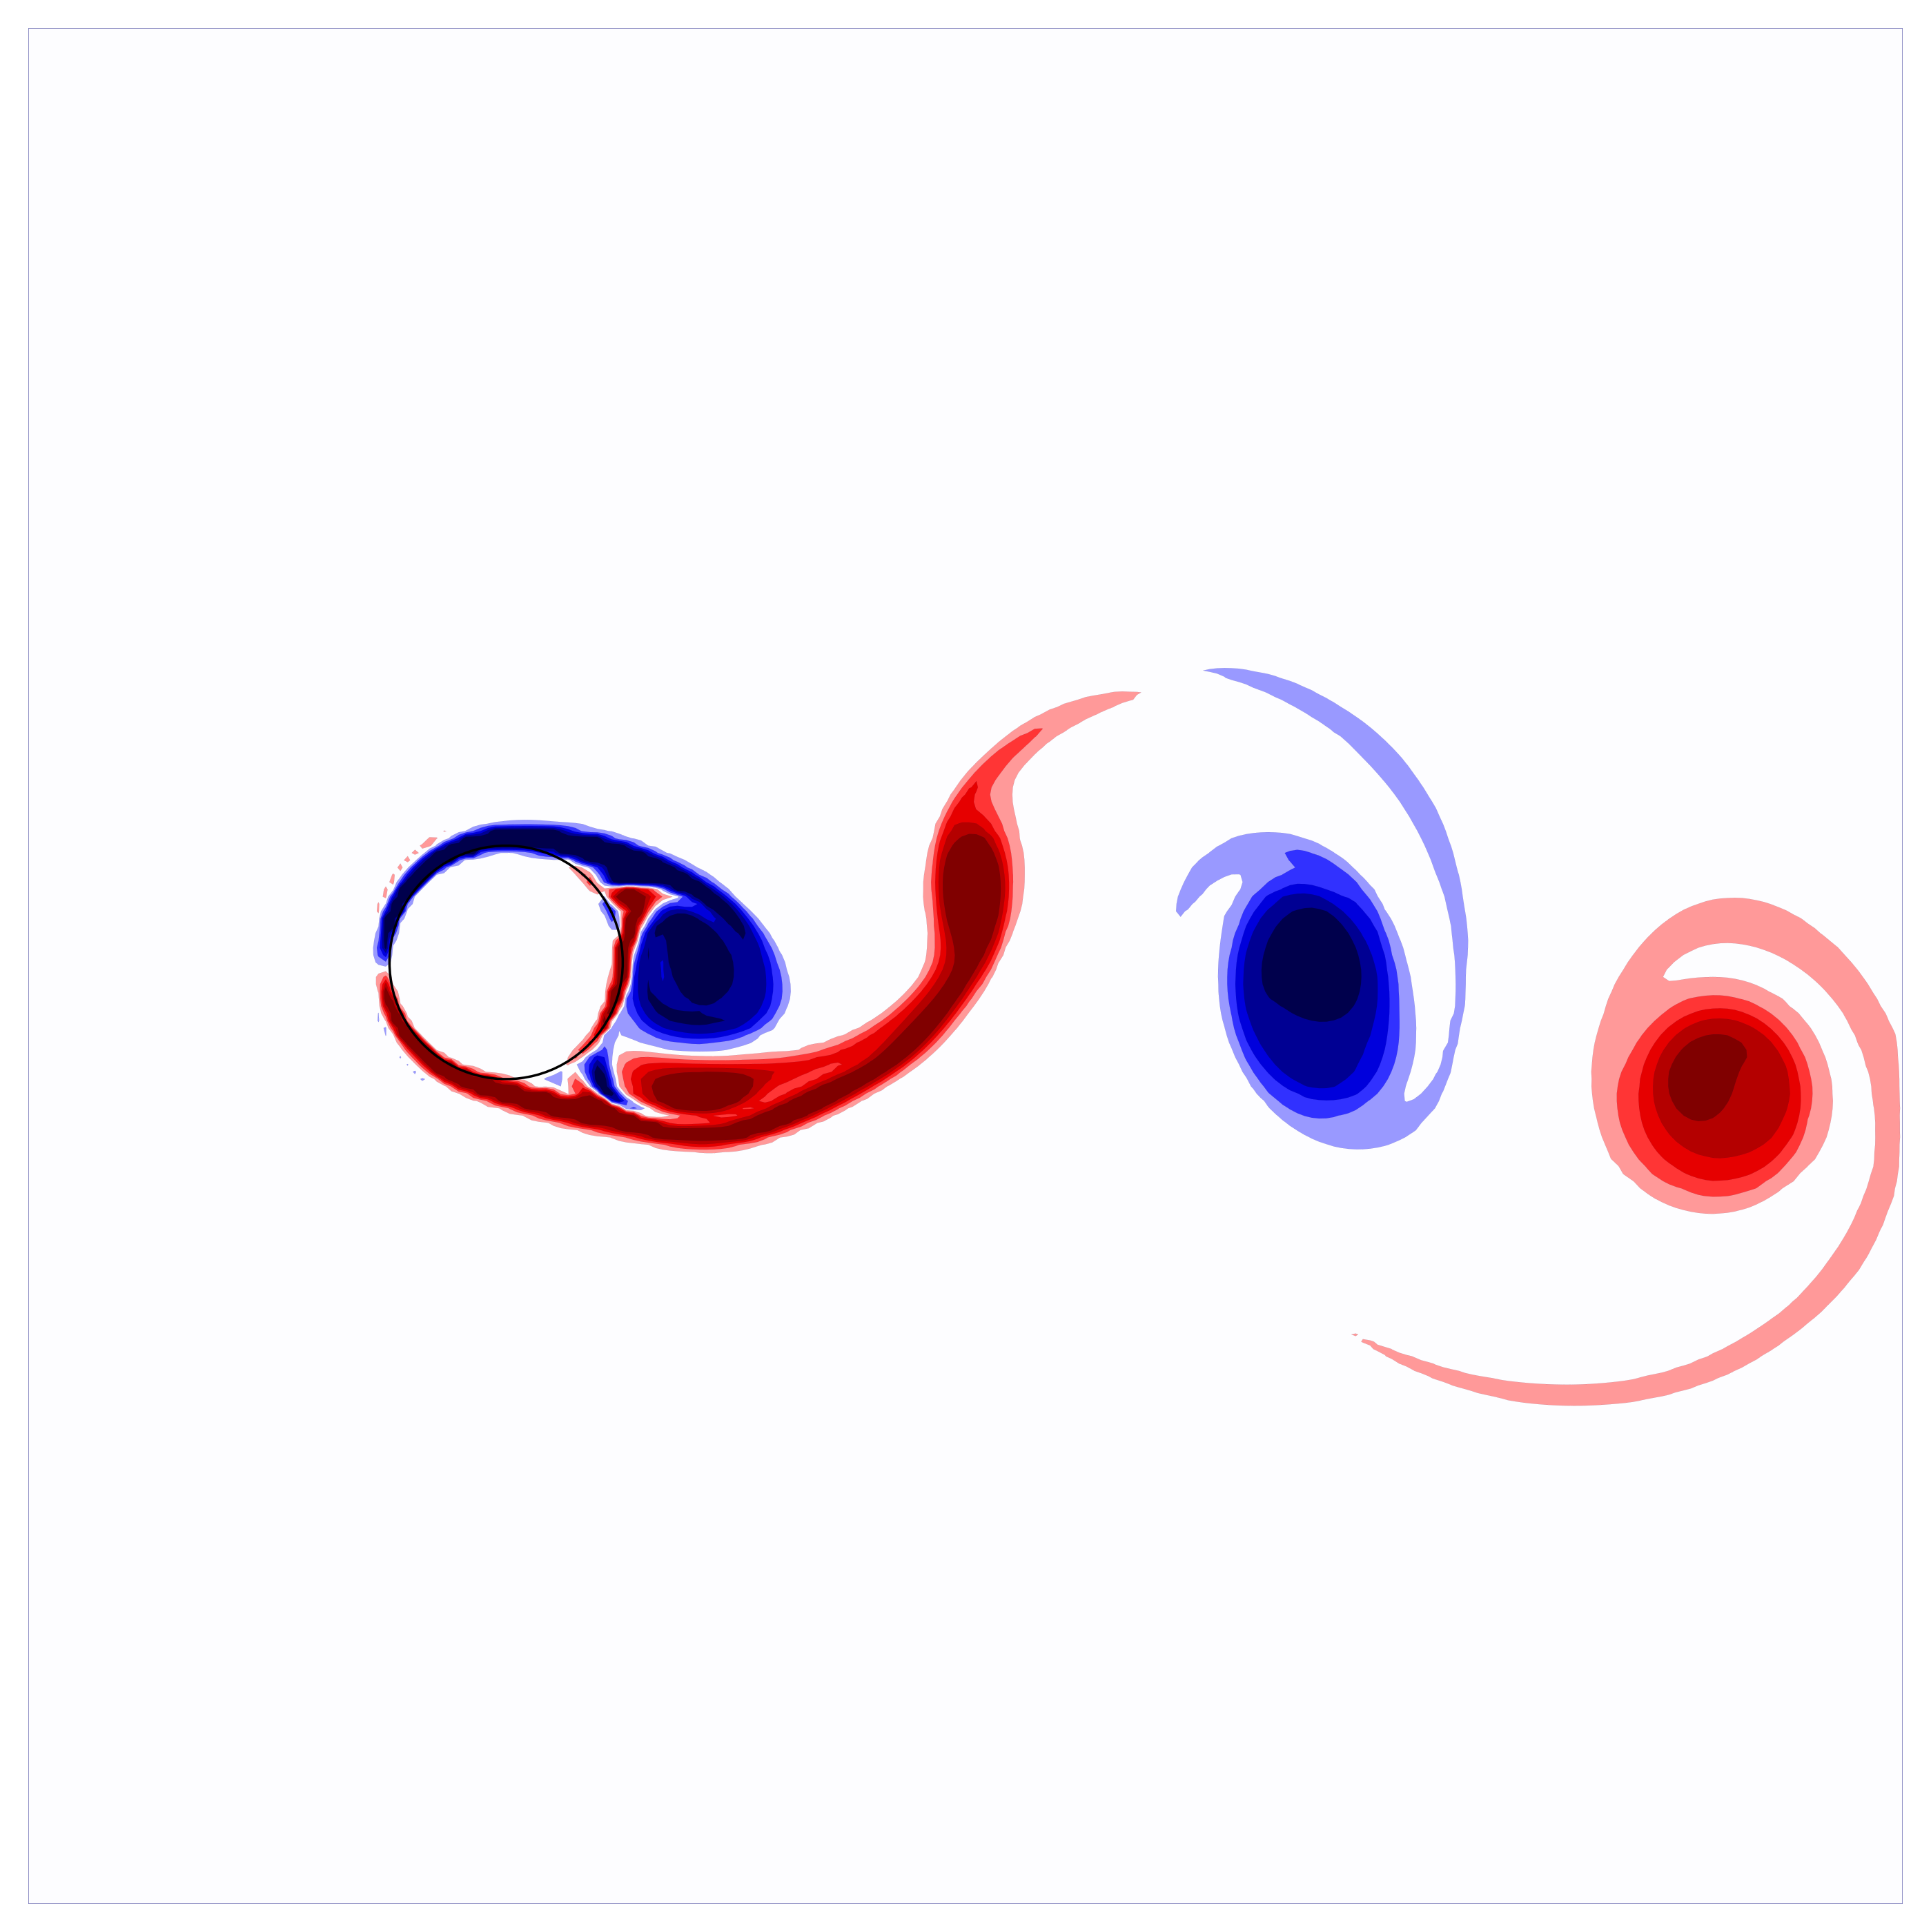
\includegraphics[width=\textwidth]{figures/Methodology/vortex_shedding/shedding_t1.5.png}
        \caption{$t^*_{n}$}
    \end{subfigure}
    \hfill
    \begin{subfigure}[b]{0.32\textwidth}
        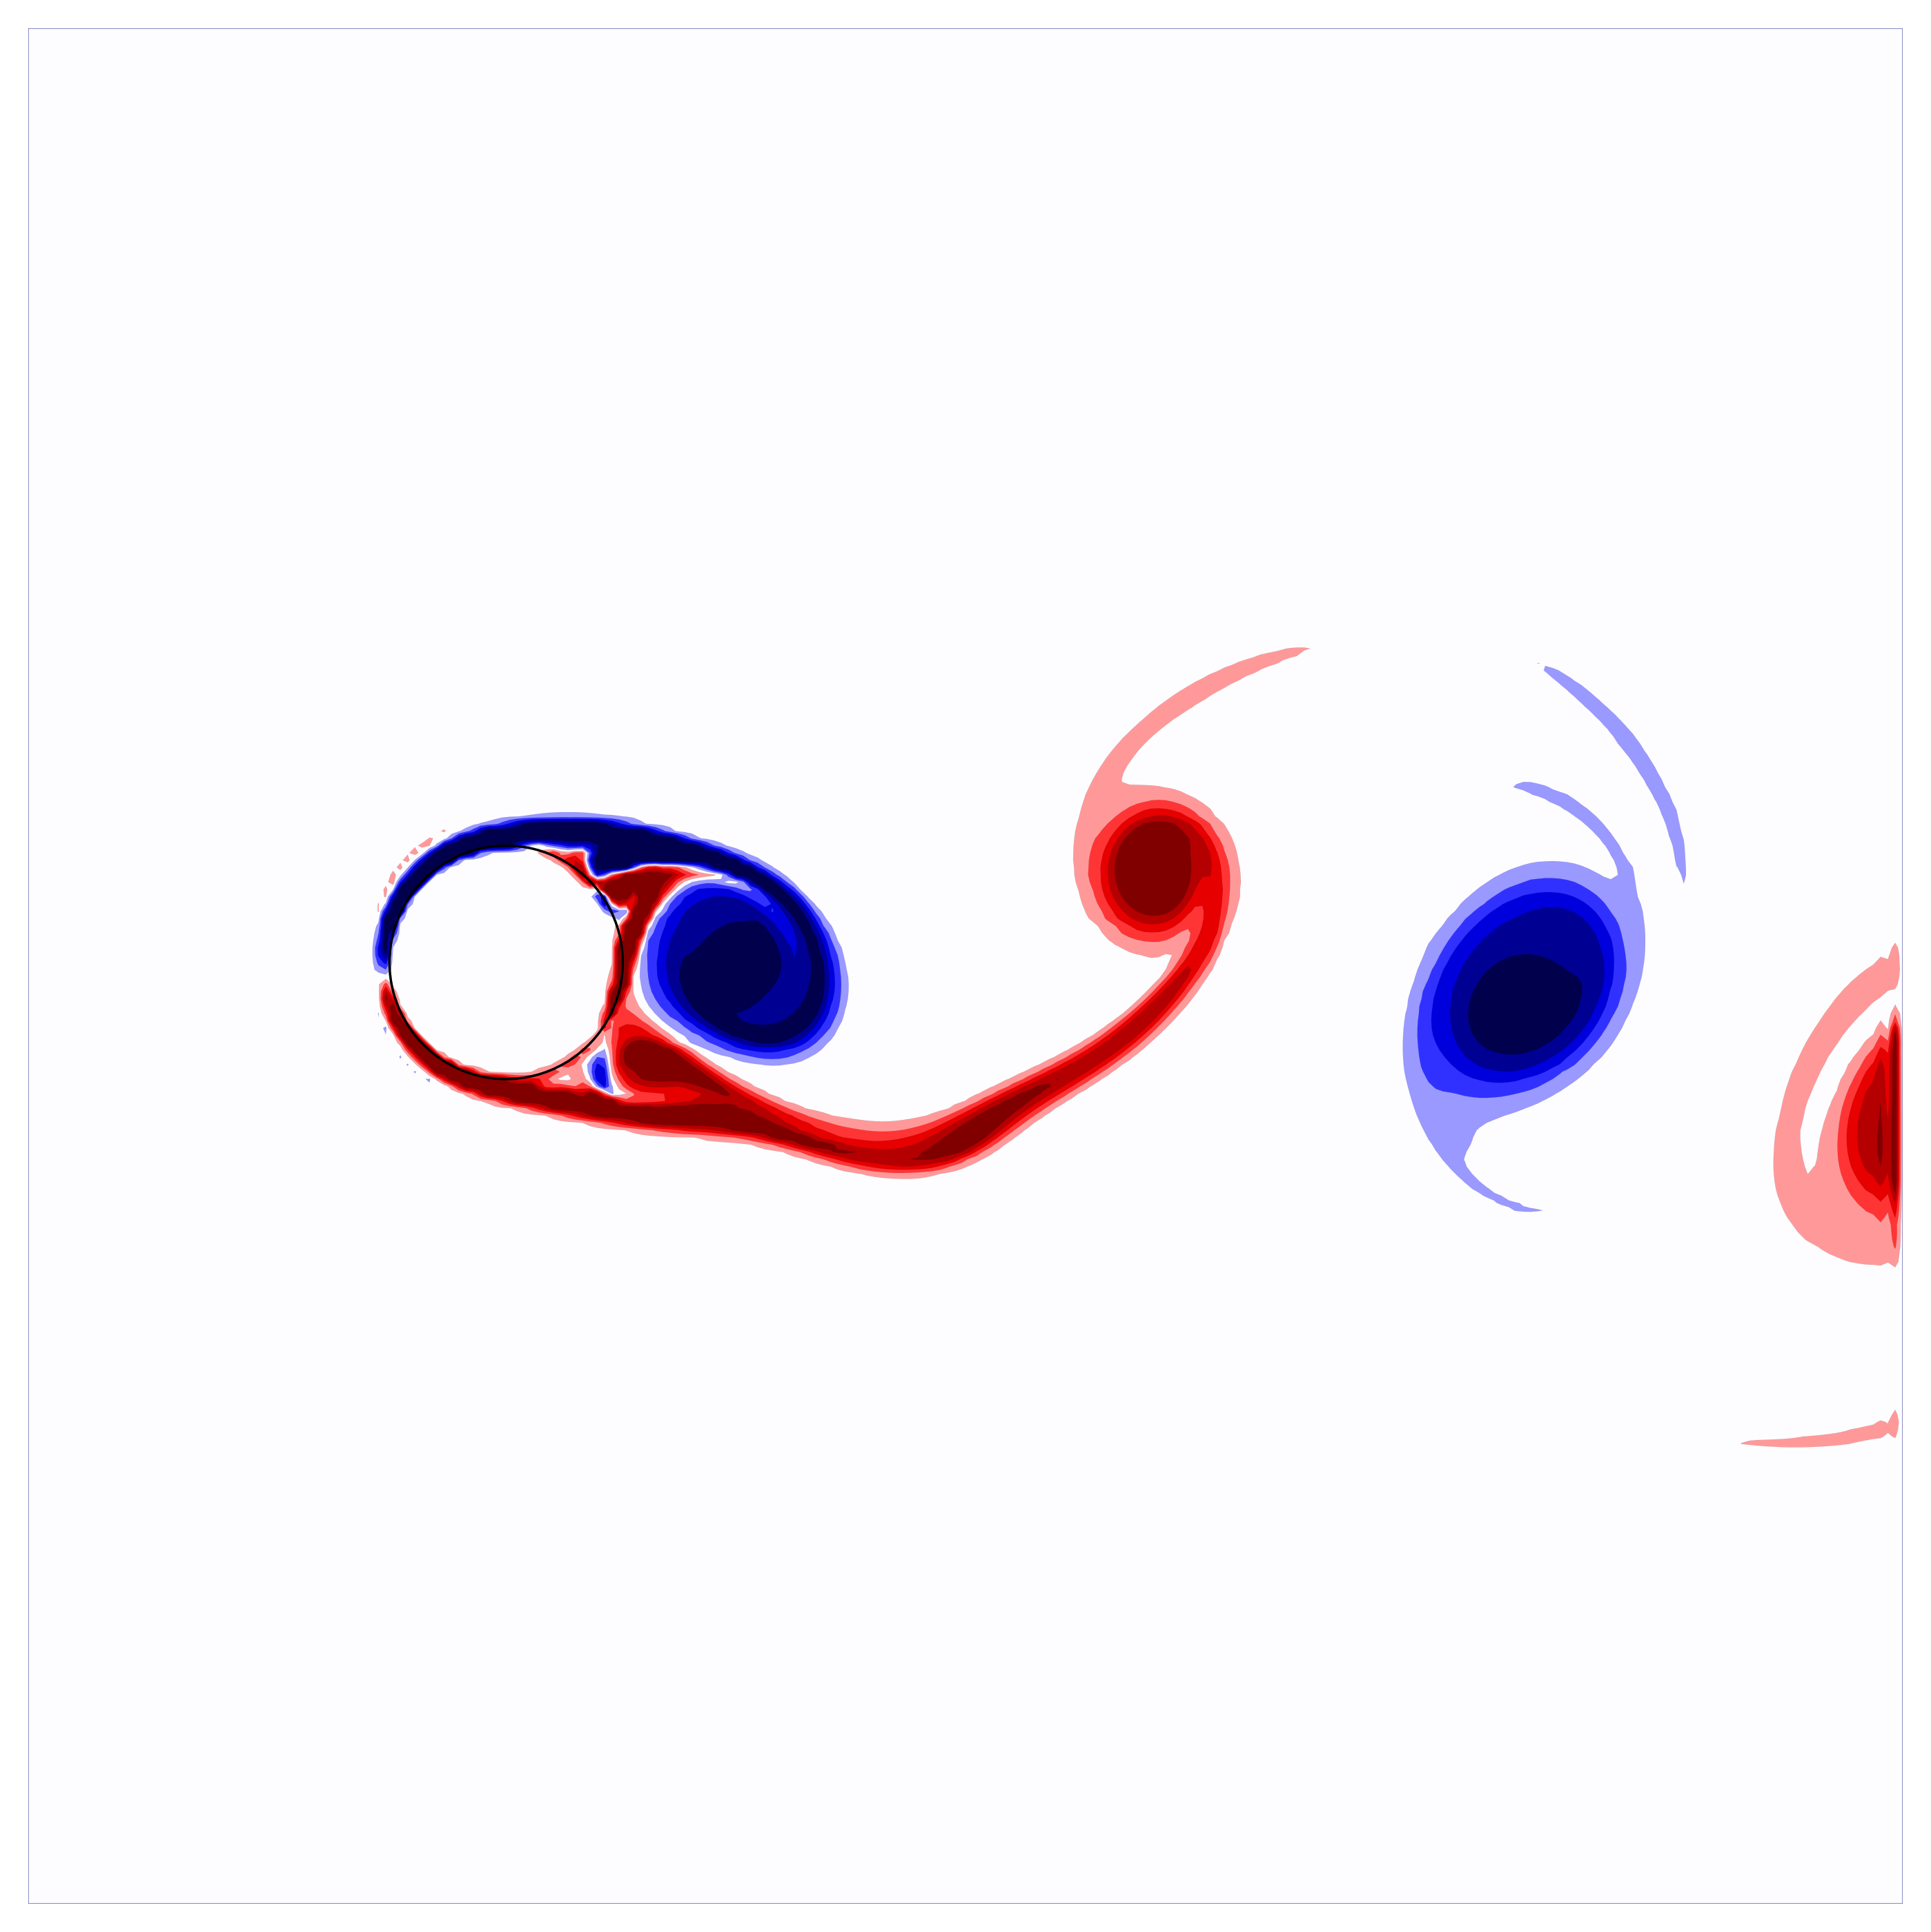
\includegraphics[width=\textwidth]{figures/Methodology/vortex_shedding/shedding_t2.5.png}
        \caption{$t^*_{n+\Delta t}$}
    \end{subfigure}
    \hfill
    \begin{subfigure}[b]{0.32\textwidth}
        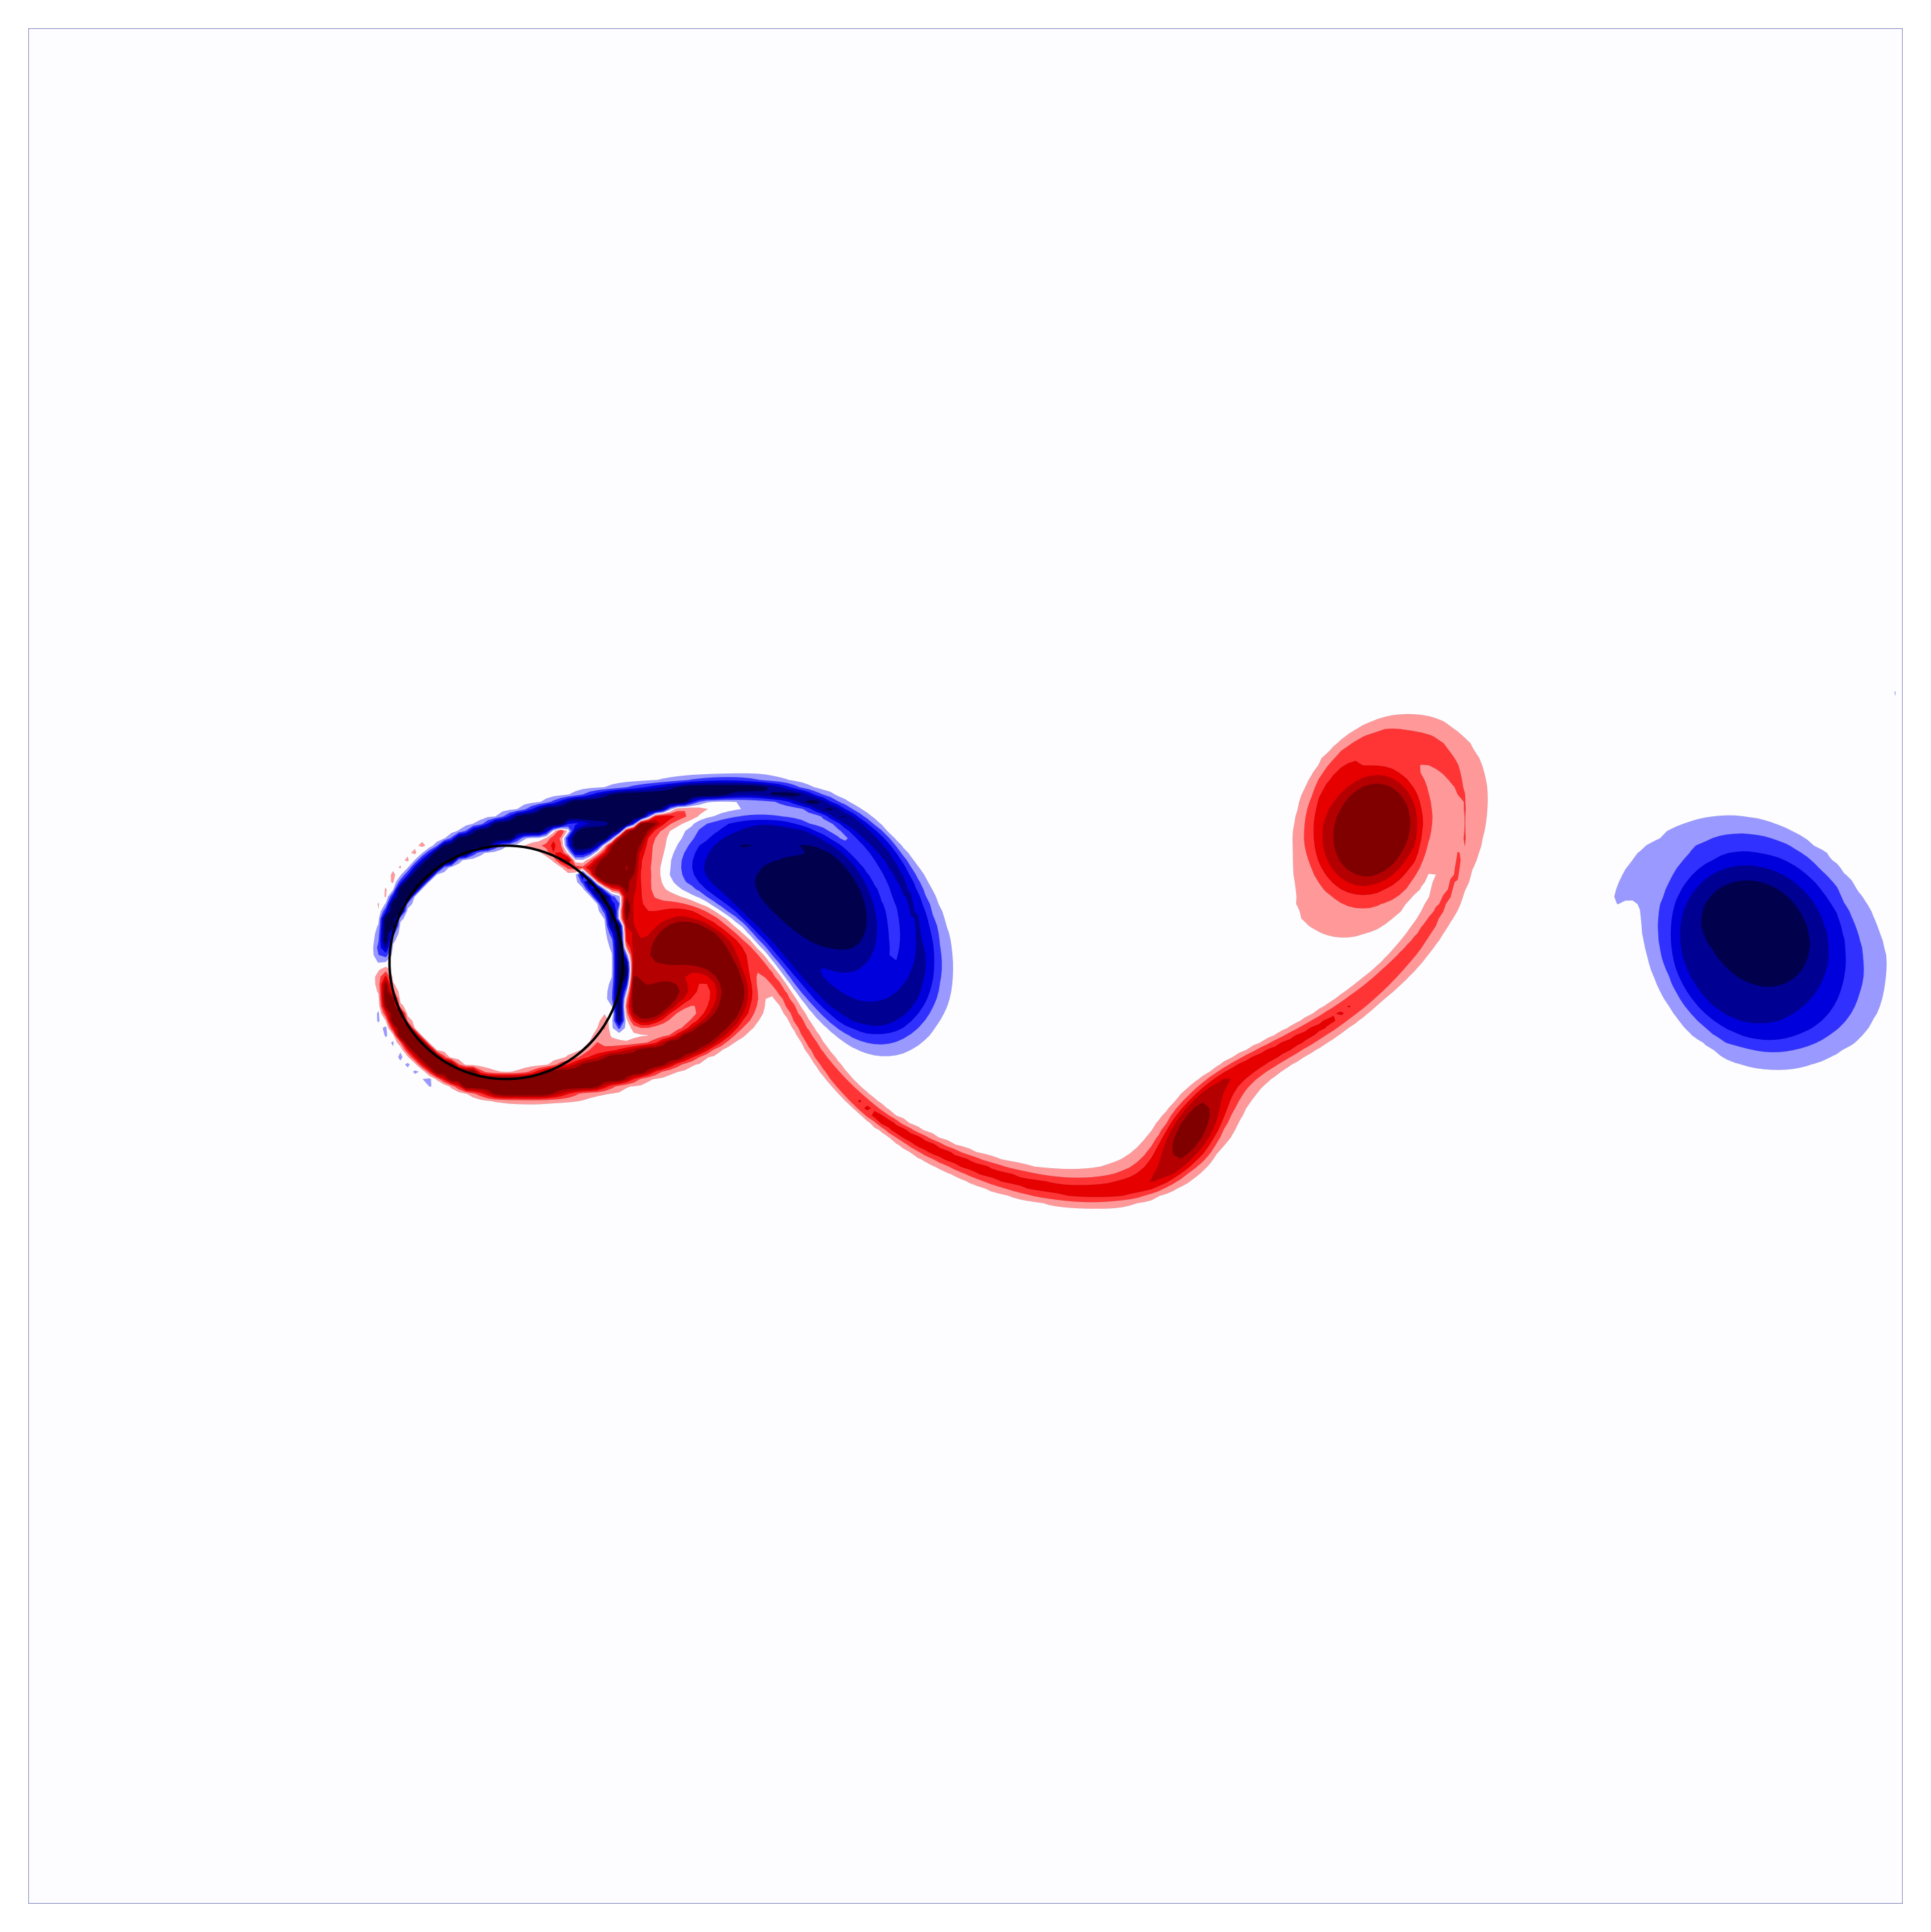
\includegraphics[width=\textwidth]{figures/Methodology/vortex_shedding/shedding_t3.5.png}
        \caption{$t^*_{n+ 2\Delta t}$}
    \end{subfigure}
    \caption{Vorticity field $\nicefrac{\omega L}{U}$ of three consecutive snapshots. Indicating positive (red) and negative (blue) vorticity. Showing the primary (large) and secondary (small) vortex structures in the wake}
    \label{fig: vortex_shedding}
\end{figure}
\todo{mss hele simulatie in appendix plaatsen}

This makes $Re=2500$ an interesting test case for the surrogate model: the dominant shedding period provides a clear, learnable periodic structure, while the secondary flow features introduce complexity and nonlinearity. This challenges the data-driven approach and motivates the inclusion of physics-informed regularisation and transfer learning capabilities in the framework. Where a lower Reynolds number would produce various length and time scales in the wake, preventing the model from properly testing its ability to capture multi-scale dynamics. The presence of these additional structures can be seen when plotting the force coefficients over time in Figure~\ref{fig: 256_forces}. 

\begin{figure}[H]
    \centering
    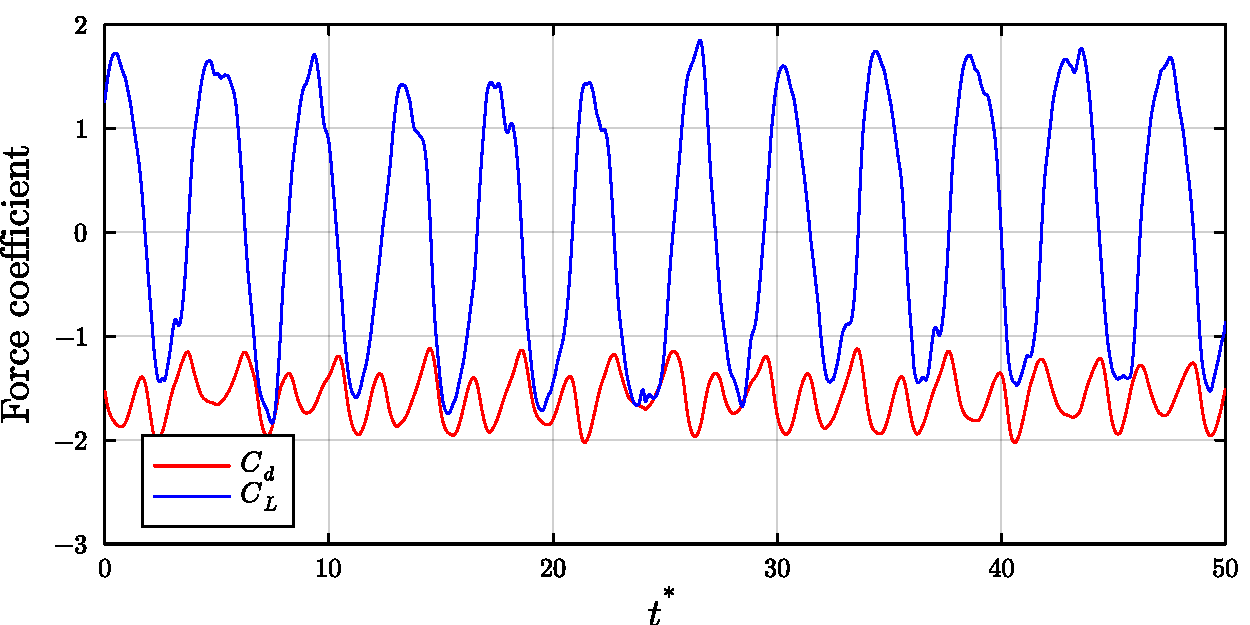
\includegraphics[width=\linewidth]{figures/Methodology/256_forces.pdf}
    \caption{lift ($C_L$) and drag coefficient ($C_D$) for 2D flow past the circular cylinder at $\mathrm{Re}=2500$, differences in amplitude and higher-frequency oscillations indicate the presence of the secondary vortex structures in the wake}
    \label{fig: 256_forces}
\end{figure}

While higher Reynolds numbers would introduce a broader spectrum of turbulent scales and further challenge the surrogate model, $Re=2500$ represents a practical upper bound given the computational constraints of this work. Increasing the Reynolds number requires a finer spatial resolution to properly resolve all relevant turbulent structures, which would rapidly increase the memory footprint and simulation wall-time. The full flow field snapshots used to train the ML framework already consume a significant portion of available memory; a further increase in resolution would exceed the practical hardware limitations of the systems used. The chosen Reynolds number, therefore, strikes a balance between flow complexity and computational practicality. 

% \subsection{Dataset Construction}

% % Structure of SimData (fields: u, p, f, μ₀, force, time, Δt, period ranges).
% % Training/test split strategy and downsampling method.

% -----------------------------------------------------------------------
\section{Data Preprocessing}
\label{sect: preprocessing}

Before being passed to the autoencoder, the raw velocity snapshots produced by WaterLily need to be preprocessed to ensure proper inference and generalisability: Removal of ghost cells, assembly of the multi-channel input tensor, and per-channel normalisation. These steps need to be applied consistently across the training, validation, and inference processes. 


\subsection{Ghost Cell Removal}
\label{sect: ghostcells}

WaterLily employs ghost cells at the domain boundary to enforce the Biot-Savart boundary conditions. These ghost cells carry values that are not physically meaningful to the flow state observations. Since we want to learn the actual underlying dynamics of the flow rather than the boundary conditions, the ghost cells are removed from the computational domain prior to training. Removing the ghost cells also has the aditional benefit that we are able to keep the amount of interior grid points as a power of 2, which will prove usefull in the parametric construction of the autoencoder. 

\begin{figure}[H]
    \centering
    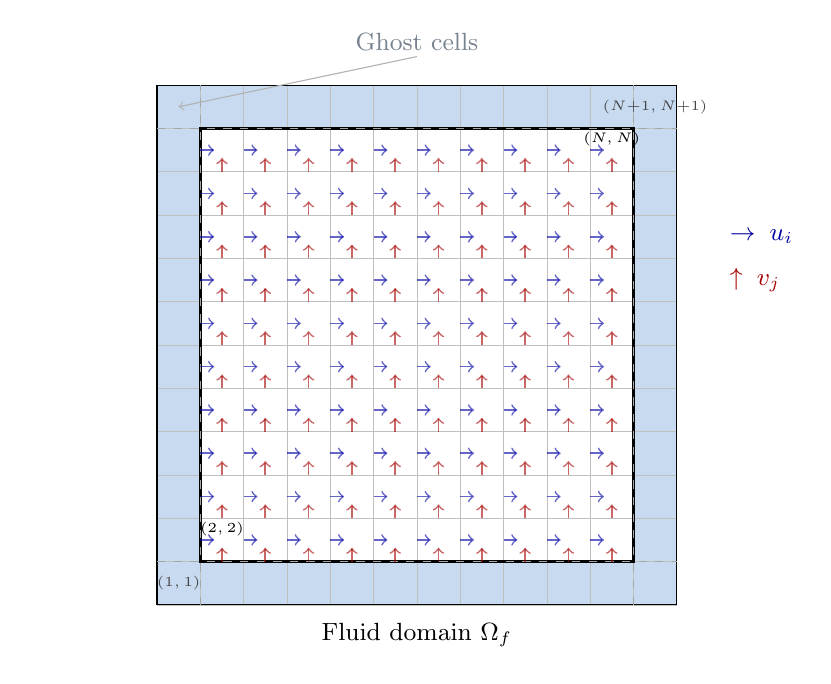
\begin{tikzpicture}[scale=1.0]

% --- parameters ---
\def\cs{0.55}    % cell size in cm

% --- colors ---
\definecolor{ghostcol}{RGB}{200,218,240}
\definecolor{interiorcol}{RGB}{255,255,255}

% --- ghost cells (full border ring) ---
\foreach \i in {0,...,11} {
    \foreach \j in {0,...,11} {
        \pgfmathparse{(\i==0 || \i==11 || \j==0 || \j==11) ? 1 : 0}
        \ifdim\pgfmathresult pt > 0pt
            \fill[ghostcol]
                (\i*\cs, \j*\cs) rectangle +(\cs,\cs);
        \fi
    }
}

% --- interior cells ---
\foreach \i in {1,...,10} {
    \foreach \j in {1,...,10} {
        \fill[interiorcol]
            (\i*\cs, \j*\cs) rectangle +(\cs,\cs);
    }
}

% --- grid lines ---
\draw[gray!50, very thin] (0,0) grid[step=\cs] (12*\cs, 12*\cs);

% --- thick border around interior domain ---
\draw[black, very thick] (1*\cs, 1*\cs) rectangle (11*\cs, 11*\cs);

% --- outer boundary ---
\draw[black, thin] (0,0) rectangle (12*\cs, 12*\cs);

% --- dashed clip lines ---
\draw[dashed, gray!70, thin] (1*\cs, 0)      -- (1*\cs,  12*\cs);
\draw[dashed, gray!70, thin] (11*\cs, 0)     -- (11*\cs, 12*\cs);
\draw[dashed, gray!70, thin] (0,      1*\cs) -- (12*\cs, 1*\cs);
\draw[dashed, gray!70, thin] (0,     11*\cs) -- (12*\cs, 11*\cs);

% --- face-centred velocity arrows (every other cell to avoid clutter) ---
% u arrows (horizontal, left face of cell)
\foreach \i in {1,...,10} {
    \foreach \j in {1,...,10} {
        \draw[->, blue!65!black, semithick, draw opacity=0.6]
            (\i*\cs, \j*\cs + 0.5*\cs) -- ++(0.32*\cs, 0);
    }
}
% v arrows (vertical, bottom face of cell)
\foreach \i in {1,...,10} {
    \foreach \j in {1,...,10} {
        \draw[->, red!65!black, semithick, draw opacity=0.6]
            (\i*\cs + 0.5*\cs, \j*\cs) -- ++(0, 0.32*\cs);
    }
}

% --- corner index labels ---
\node[font=\tiny, gray!55!black] at (0.5*\cs, 0.5*\cs)   {$(1,1)$};
\node[font=\tiny, gray!55!black] at (11.5*\cs, 11.5*\cs) {$(N{+}1,N{+}1)$};
\node[font=\tiny, black]         at (1.5*\cs,  1.75*\cs)  {$(2,2)$};
\node[font=\tiny, black]         at (10.5*\cs, 10.75*\cs) {$(N,N)$};

% --- annotations ---
\node[font=\small, align=center] at (6*\cs, -0.7*\cs)
    {Fluid domain $\Omega_f$};

\node[font=\small, ghostcol!60!black, fill=white, inner sep=2pt]
    (glabel) at (6*\cs, 13.0*\cs) {Ghost cells};
\draw[->, gray!60, thin] (glabel.south) -- (0.5*\cs, 11.5*\cs);

% --- legend ---
\node[font=\small, blue!65!black, anchor=west]
    at (13.0*\cs, 8.5*\cs) {$\rightarrow\; u_i$};
\node[font=\small, red!65!black,  anchor=west]
    at (13.0*\cs, 7.5*\cs) {$\uparrow\; v_j$};

\node[font=\small, white, anchor=west]
    at (-3*\cs, 8.5*\cs) {$\rightarrow\; u_i$};
\node[font=\small, white,  anchor=west]
    at (-3*\cs, 7.5*\cs) {$\uparrow\; v_j$};

\end{tikzpicture}
    \caption{Illustration of the WaterLily grid showing the location of ghost cells }
    \label{fig: ghost cells}
\end{figure}

The ghost cells are removed by slicing the raw arrays from index $2$ to $N$ in each spatial dimension, yielding interior fields of size $N_x \times N_y$ for both the velocity field $\mathbf{u}\in \mathbb{R}^{N_x\times N_y \times N_u}$ and the zeroth kernel moment  $\boldsymbol{\mu_0} \in \mathbb{R}^{N_x \times N_y \times N_u}$, where $N_x$ and $N_y$ are the number of grid cells, and $N_u$ is the number of velocity components.

\subsection{Channel Construction}
\label{subsect: channels}

The model is provided with explicit geometric information about the simulation domain by concatenating the zeroth kernel moment $\boldsymbol{\mu_0}$ to the velocity field $\mathbf{u}$ along the channel dimension, forming the input tensor

\begin{equation}\label{eq:input_tensor}
    \mathbf{x}_\text{in} = [\mathbf{u}\, ;\, \boldsymbol{\mu_0}] \in 
    \mathbb{R}^{N_x \times N_y \times C_\text{in}}.
\end{equation}

For our 2D simulation, each training sample therefore consists of a 4-channel input tensor and a 2-channel reconstruction target. The reconstruction target is the velocity field $\mathbf{u}$, containing the $x$- and $y$-components of velocity. 

Since $\boldsymbol{\mu_0}$ is unity in the fluid and zero inside the solid, its inclusion provides the encoder with explicit geometric context, allowing it to produce latent representations that are informed on the simulation geometry. The decoder reconstructs only the 2-channel velocity field $\hat{\mathbf{u}}$; predicting $\boldsymbol{\mu_0}$ is unnecessary since, in the absence of fluid-structure interaction, the body velocity is fully determined by Equation~\ref{eq: WaterLilyBodyVelocity} and therefore known at any time $t^*$.


\subsection{Normalization}
\label{sect: normalization}

% Per-channel z-score normalization scheme.
% Where statistics are computed, how the Normalizer is stored, and how the inverse transform is applied at decode time.

% -----------------------------------------------------------------------
\section{Autoencoder}
\label{sect: AE}

To harness the Neural ODE's predictive capabilities, we need a way to reduce the dimensionality of our dynamical system. This is the role the autoencoder encompasses: it provides a way to produce a compact, non-linear representation of the instantaneous flow state on which the latent dynamics can subsequently be learned. A convolutional Autoencoder is well-suited to this task, as its filters are designed to extract local spatial features from grid-structured fields, while the implementation of non-linear activation functions allows it to represent the flow states on a curved low-dimensional manifold. 

The autoencoder learns an efficient reduced-order representation of the instantaneous full-order flow state. The AE consists of two parts, namely an encoder and a decoder. The encoder $\varphi_\theta: \mathbb{R}^{N_x \times N_y \times C_{in}} \to \mathbb{R}^{N_z}$, maps the instantaneous full-order augmented input to a latent state vector $\mathbf{z} = \varphi_\theta(\mathbf{x}_\text{in})$, with small dimensions such that $N_z \ll N_x N_y C_\text{in}$. The decoder $\psi_\theta : \mathbb{R}^z \to \mathbb{R}^{N_x \times N_y \times N_u}$ then maps this latent state vector back to physical space $\hat{\mathbf{u}} = \psi_\theta(\mathbf{z})$ with the following goal.


\begin{equation}\label{eq: AE_goal}
    \hat{\mathbf{u}} \simeq \mathbf{u}, \quad \text{where} \quad 
    \hat{\mathbf{u}} = \psi_\theta(\mathbf{z}), \quad 
    \mathbf{z} = \varphi_\theta(\mathbf{x}_\text{in})
\end{equation}


% Encoding 256×256×4 flow fields to a 16-dimensional latent space.

\subsection{Architecture}
\label{sect: AEarch}

The encoder and decoder are constructed parametrically from a small set of hyperparameters: the number of convolutional blocks $n_\text{conv}$, the number of dense layers $n_\text{dense}$, the base channel count $C_\text{base}$, the convolution kernel size $k$, the pooling kernel size $p$, and the latent dimension $N_z$. Which are all summarised in Table~\ref{tab: ae_hyperparameters}.

\begin{table}[H]
    \centering
    \begin{tabular}{@{}llc@{}}
        \toprule
        Symbol & Description  \\
        \midrule
        $n_\text{conv}$    & Number of convolutional blocks per encoder/decoder    \\
        $n_\text{dense}$   & Number of fully-connected layers per encoder/decoder  \\
        $C_\text{base}$    & Base channel count (first encoder block)              \\
        $k$                & Convolution kernel size                               \\
        $p$                & Pooling/upsampling kernel size                        \\
        $s$                & Convolution stride                                    \\
        $N_z$              & Latent dimension                                      \\
        \bottomrule
    \end{tabular}
    \caption{Governing hyperparameters for parametric autoencoder construction}
    \label{tab: ae_hyperparameters}
\end{table}


An illustrative overview of the autoencoder architecture with these hyperparameters is shown in Figure~\ref{fig: AE}, which shows how the encoder, dense bottleneck, and decoder connect to form the full compression-decompression pipeline. The following subsections will discuss the architecture of these components individually. 


\begin{figure}[H]
    \centering
    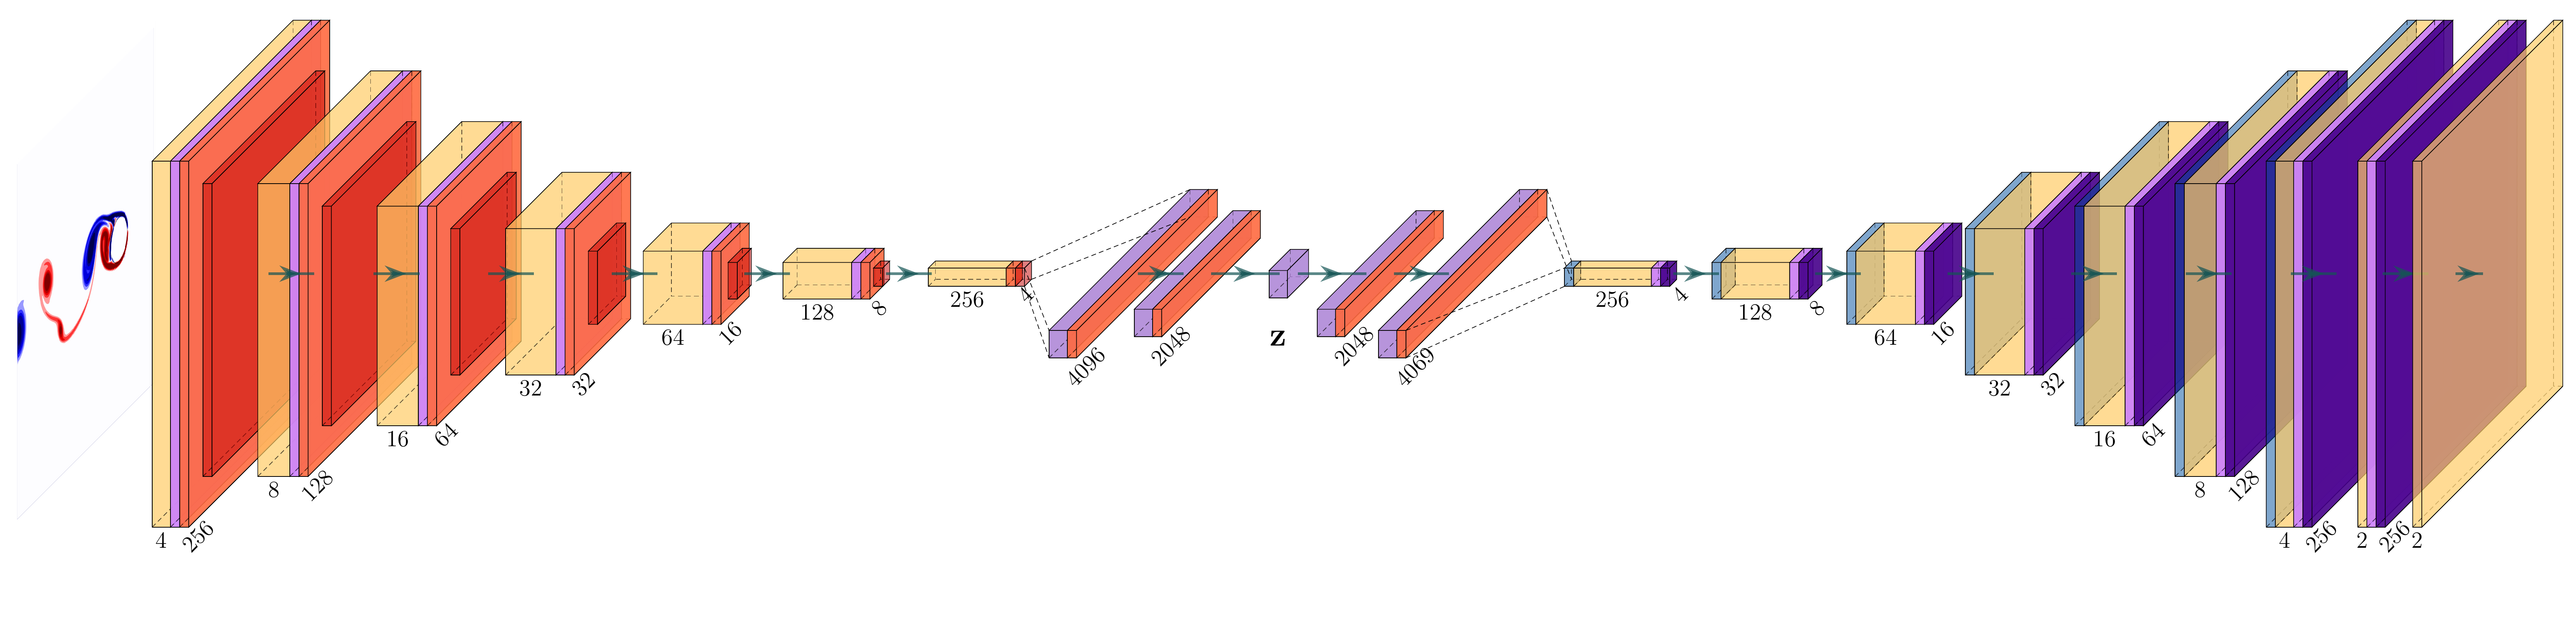
\includegraphics[width=\linewidth]{figures/Methodology/autoencoder.png}
    \caption{Schematic view of the CNN-AE architecture with $n_\text{conv}=6$, $n_\text{dense}=2$, $C_\text{base}=8$, $k=3$, $p=2$, $s=1$, $N_z=16$ and $C_\text{in}=4$. The colour coding for each layer is:
  2D-convolution: \colorbox{\ConvColor}{\phantom{x}},
  Batch normalization: \colorbox{\BnColor}{\phantom{x}},
  ReLU activation: \colorbox{\ReluColor}{\phantom{x}},
  max pooling: \colorbox{\PoolColor}{\phantom{x}},
  fully-connected layer: \colorbox{\FcColor}{\phantom{x}},
  GELU activation: \colorbox{\GeluColor}{\phantom{x}},
  compressed feature map:~\colorbox{\FeatColor}{\phantom{x}},
  upsampling: \colorbox{\UnpoolColor}{\phantom{x}}}
    \label{fig: AE}
\end{figure}

\subsubsection{Encoder}

The encoder consists of $n_\text{conv}$ stacked compression blocks, followed by a sequence of $n_\text{dense}$ fully connected layers that project the flattened feature maps onto the latent vector $\mathbf{z} \in \mathbb{R}^{N_z}$. Each compression block applies, in order, a 2D convolution with kernel size $k$ and stride $s$, a batch-normalisation layer, a ReLU activation, and a $p \times p$ max-pooling operation. Same-padding is used in every convolution so that spatial resolution is reduced only through the pooling step. The convolution extracts local spatial features from the instantaneous flow state, and batch normalisation stabilises the distribution of layer inputs across a mini-batch. Batch normalisation stabilises training by smoothing the loss landscape, scaling and shifting the layer inputs based on trainable parameters to preserve model expressivity \cite{Santurkar2019}, allowing larger learning rates and reducing sensitivity to weight initialisation. ReLU introduces the non-linearity to represent the flow states on a low-dimensional latent space. 

\begin{figure}[h]
    \centering
    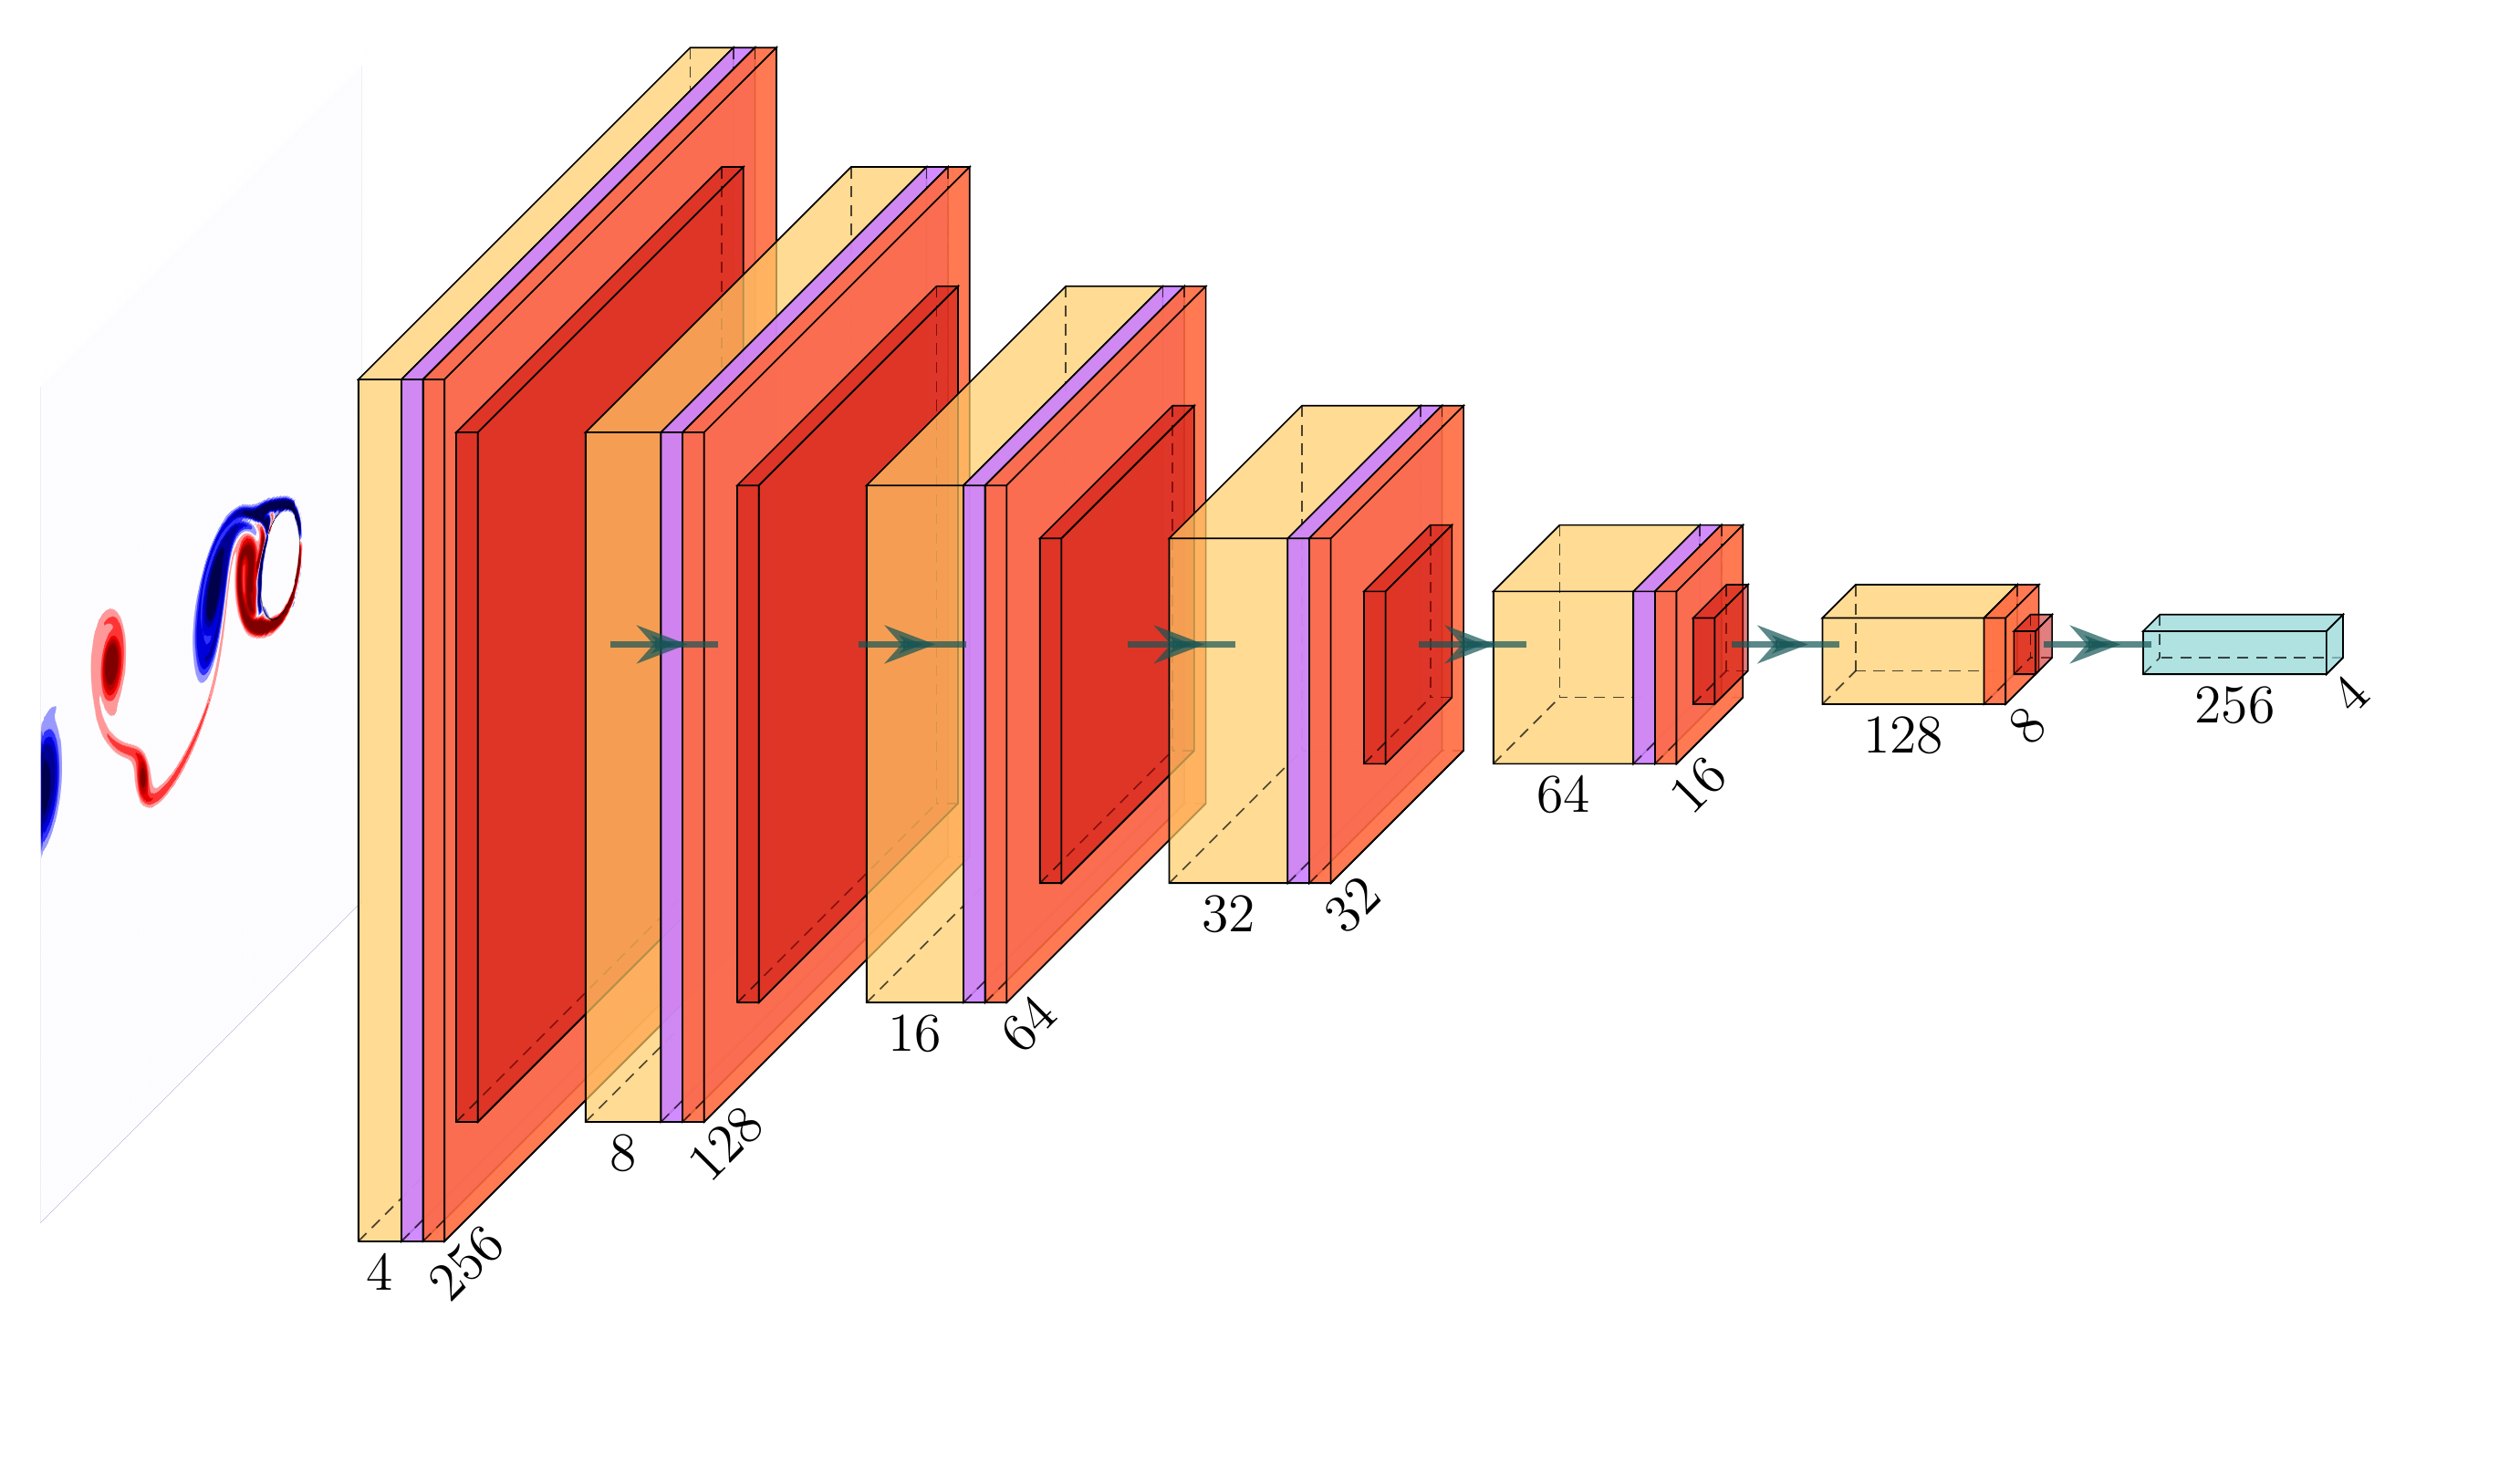
\includegraphics[width=\linewidth]{figures/Methodology/encoder.png}
    \caption{Example encoder architecture with $n_\text{conv}=6$, $p=2$, $k=3$, $C_\text{in}=4$ and $C_\text{base}=8$. The colour coding for each layer is:
  2D-convolution:~\colorbox{\ConvColor}{\phantom{x}},
  Batch normalization:~\colorbox{\BnColor}{\phantom{x}},
  ReLU activation:~\colorbox{\ReluColor}{\phantom{x}},
  max pooling:~\colorbox{\PoolColor}{\phantom{x}}} \&
  compressed feature map:~\colorbox{\FeatColor}{\phantom{x}}
    \label{fig: encoder}
\end{figure}

The encoder achieves its compression by doubling the channel count after each block and halving the spatial resolution using the maxpool operation, shown mathematically in \ref{eq: ae_channels} \& \ref{eq: ae_spatial}. This means that at each convolutional step, the number of feature maps is doubled to extract more information from the turbulent flow snapshot, while at each downsampling step, the dimension is reduced to allow the next layer to combine the identified flow features into a new feature map. This allows the extraction of larger and more complex features for progressively deeper convolutional networks from simple non-linear combinations of the previous ones \cite{Eivazi2022}.

\begin{align}
    C_i &= C_\text{base}\, 2^{\,i-1}, & i &= 1, \dots, n_\text{conv}, 
    \label{eq: ae_channels} \\
    H_i &= N_x / p^{\,i}, \qquad W_i = N_y / p^{\,i}, & i &= 1, \dots, n_\text{conv}.
    \label{eq: ae_spatial}
\end{align}

 These deeper feature maps, therefore, encode larger-scale flow structures, such as the periodic wake pattern, while the shallow maps retain local features such as shear layers and boundary-layer gradients. The final compression block omits the batch normalisation step to preserve the activation magnitudes that feed into the dense bottleneck. An example schematic of an encoder is shown in Figure~\ref{fig: encoder}, showing how the reduction in spatial size is achieved while increasing the number of channels.


\subsubsection{Dense layers}

After the final compression block, the feature map of dimensions $H_{n_\text{conv}} \times W_{n_\text{conv}} \times C_{n_\text{conv}}$ is flattened and passed through a sequence of $n_\text{dense}$ fully connected layers. Each successive layer halves the number of nodes, with the last layer projecting onto the $N_z$-dimensional latent vector $\mathbf{z} = \varphi_\theta(\mathbf{x}_\text{in})$ shown in Figure~\ref{fig: dense}.

\begin{figure}[H]
    \centering
    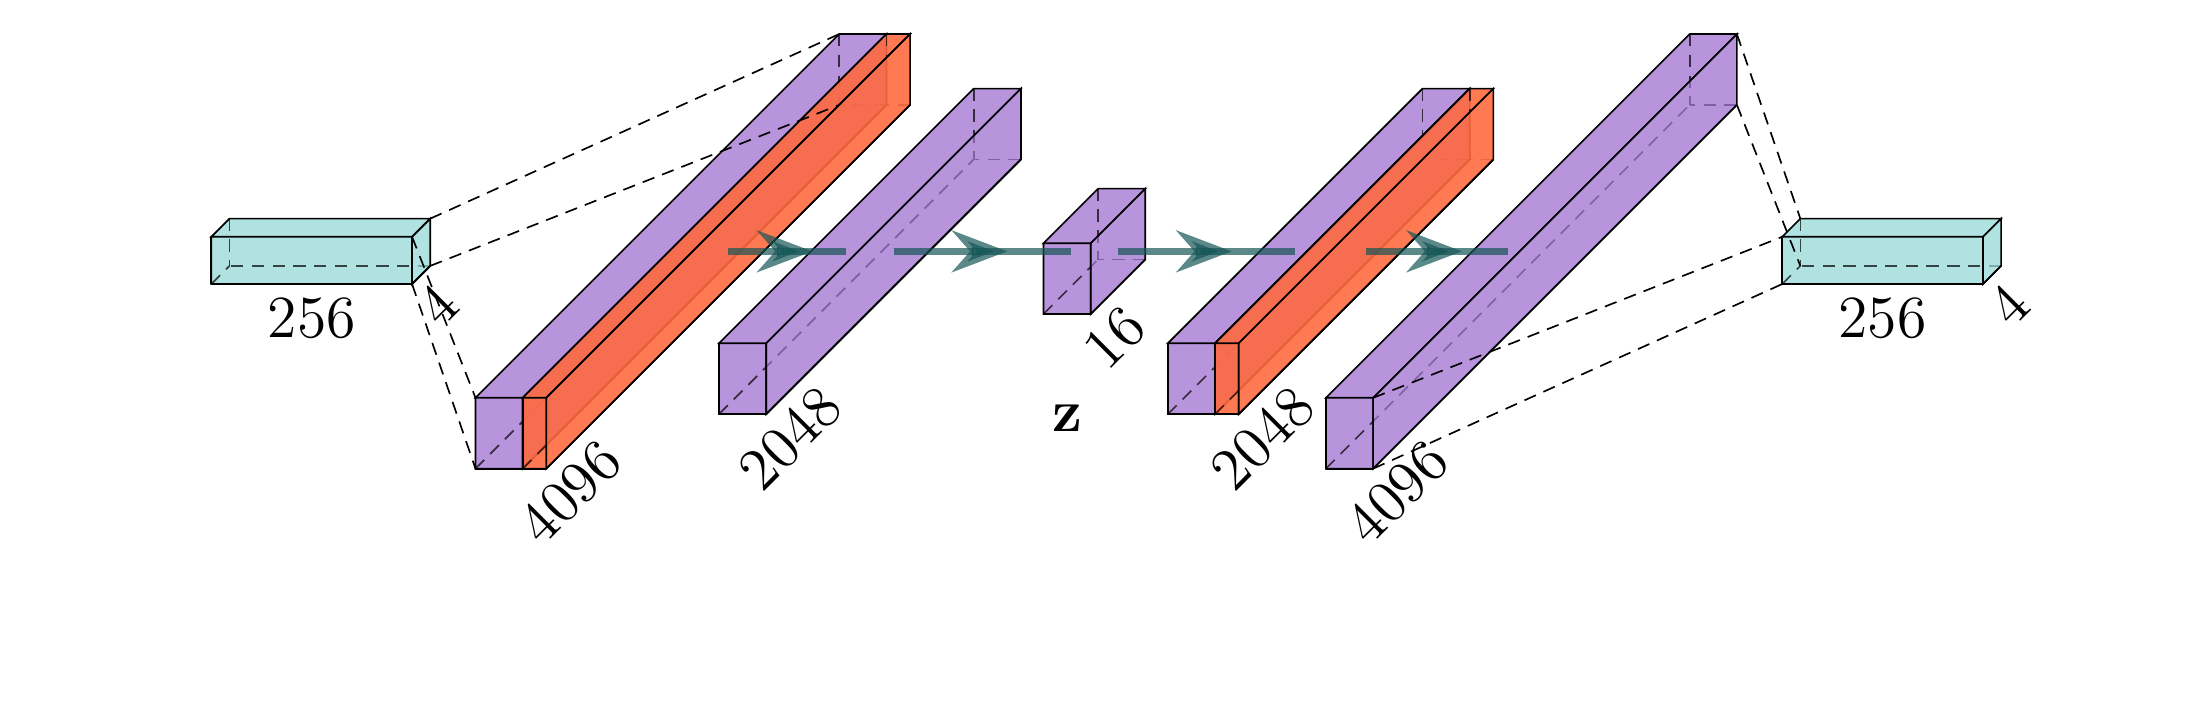
\includegraphics[width=\linewidth]{figures/Methodology/latent.png}
    \caption{Example of the dense compression/decompression with $n_\text{dense}=2$ and a latent size of 16. The colour coding for each layer is: ReLU activation: \colorbox{\ReluColor}{\phantom{x}},
    fully-connected~layer: \colorbox{\FcColor}{\phantom{x}} \&
    compressed feature map:~\colorbox{\FeatColor}{\phantom{x}}}
    \label{fig: dense}
\end{figure}

The dense bottleneck performs the bulk of the dimensionality reduction: the convolutional blocks reorganise the input into a compact representation with a large number of channels, and the dense layers then learn a non-linear projection from this representation to the low-dimensional space of the latent state. No activation function is applied to the final dense layer, so that the latent vector $\mathbf{z}$ is unconstrained in $\mathbb{R}^{N_z}$ rather than being constrained by an activation function. This ensures that the Neural ODE operates on the same unconstrained domain as the encoder. 

The latter half of the dense bottleneck mirrors the first half, projecting $\mathbf{z}$ back to the same dimensions as the last dense layer of the dense encoder. After this, it doubles the number of nodes at each successive layer until the original flattened feature map size $H_{n_\text{conv}} \cdot W_{n_\text{conv}} \cdot C_{n_\text{conv}}$ is recovered, with ReLU activations between layers. The resulting vector is then reshaped into a feature map of dimensions $H_{n_\text{conv}} \times W_{n_\text{conv}} \times C_{n_\text{conv}}$, serving as the starting point for the decompression blocks.

\subsubsection{Decoder}

The decoder $\psi_\theta$ reverses the operation done by the encoder by passing the feature map at the end of the dense bottleneck and passing it through $n_\text{conv}$ decompression blocks, each of which consists of a bilinear upsampling by a factor of $p$, a 2D convolution with kernel size $k$ and stride $s$, and a GELU activation. 

\begin{figure}[H]
    \centering
    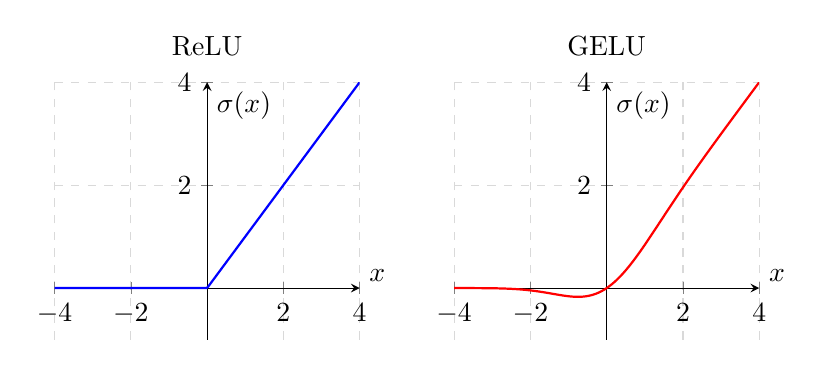
\begin{tikzpicture}
        \begin{axis}[
            name=relu,
            width=0.45\linewidth,
            height=0.4\linewidth,
            xmin=-4, xmax=4,
            ymin=-1, ymax=4,
            axis lines=middle,
            xlabel={$x$},
            ylabel={$\sigma(x)$},
            xlabel style={at={(axis description cs:1.0,0.25)}, anchor=west},
            ylabel style={at={(axis description cs:0.5,1.0)}, anchor=north west},
            xtick={-4,-2,2,4},
            ytick={2,4},
            samples=200,
            domain=-4:4,
            title={ReLU},
            grid=major,
            grid style={dashed, gray!30},
        ]
            \addplot[blue, thick] {max(0,x)};
        \end{axis}

        \begin{axis}[
            at={(relu.east)}, anchor=west, xshift=1.2cm,
            width=0.45\linewidth,
            height=0.4\linewidth,
            xmin=-4, xmax=4,
            ymin=-1, ymax=4,
            axis lines=middle,
            xlabel={$x$},
            ylabel={$\sigma(x)$},
            xlabel style={at={(axis description cs:1.0,0.25)}, anchor=west},
            ylabel style={at={(axis description cs:0.5,1.0)}, anchor=north west},
            xtick={-4,-2,2,4},
            ytick={2,4},
            samples=200,
            domain=-4:4,
            title={GELU},
            grid=major,
            grid style={dashed, gray!30},
        ]
            \addplot[red, thick] {0.5*x*(1 + tanh(sqrt(2/pi)*(x + 0.044715*x^3)))};
        \end{axis}
    \end{tikzpicture}
    \caption{Comparison of the ReLU and GELU activation functions. ReLU zeroes out all negative inputs, while GELU smoothly gates negative inputs near zero and asymptotes to the identity for large positive inputs.}
    \label{fig: activations}
\end{figure}

The upsampling step reverses the spatial compression introduced by the encoder's pooling operation, aiming to restore the latent vector to its full physical dimensions. The subsequent convolution learns a smooth refinement of the upsampled feature map. In contrast to the encoder's ReLU activation function, the decoder uses GELU activation because the reconstructed velocity field contains both positive and negative values, and ReLU's hard zero clipping would restrict the reconstruction of the negative-velocity regions of the wake. Where GELU allows the decompression blocks to produce negative variables, such that periodic flow features can be properly reconstructed, Figure~\ref{fig: activations} shows a graphic comparison of these two activation functions. 

\begin{align}
    C_i &= C_\text{base}\, 2^{\,n_\text{conv}-i}, & i &= 1, \dots, n_\text{conv},
    \label{eq: ae_dec_channels} \\
    H_i &= N_x \cdot p^{\,i-n_\text{conv}}, \qquad W_i = N_y \cdot p^{\,i-n_\text{conv}}, & i &= 1, \dots, n_\text{conv}.
    \label{eq: ae_dec_spatial}
\end{align}

In the decoder, the decompression blocks halve the channel count while doubling the spatial dimension in a symmetrical fashion to the encoders' compression path, shown in \ref{eq: ae_dec_channels} \& \ref{eq: ae_dec_spatial}. The final decompression block is followed by two additional convolutional operations, seen on the right in Figure~\ref{fig: decoder}. The first of these applies a $k \times k$ convolution that maps the last decoder channel count, which is the same as the input channel count in the encoder $C_\text{in}$, to $N_u$, so that they match the dimensions of the target velocity field. The second layer applies another $k \times k$ convolution with $N_u \to N_u$ channels and acts as a learned smoothing layer, which aims to suppress checkerboarding \todo{add source on the checkerboarding} artefacts that can be produced by repeated bilinear upsampling. Both of these last layers have linear activation functions, so the reconstructed velocity field is a linear combination of the last feature map. 


\begin{figure}[H]
    \centering
    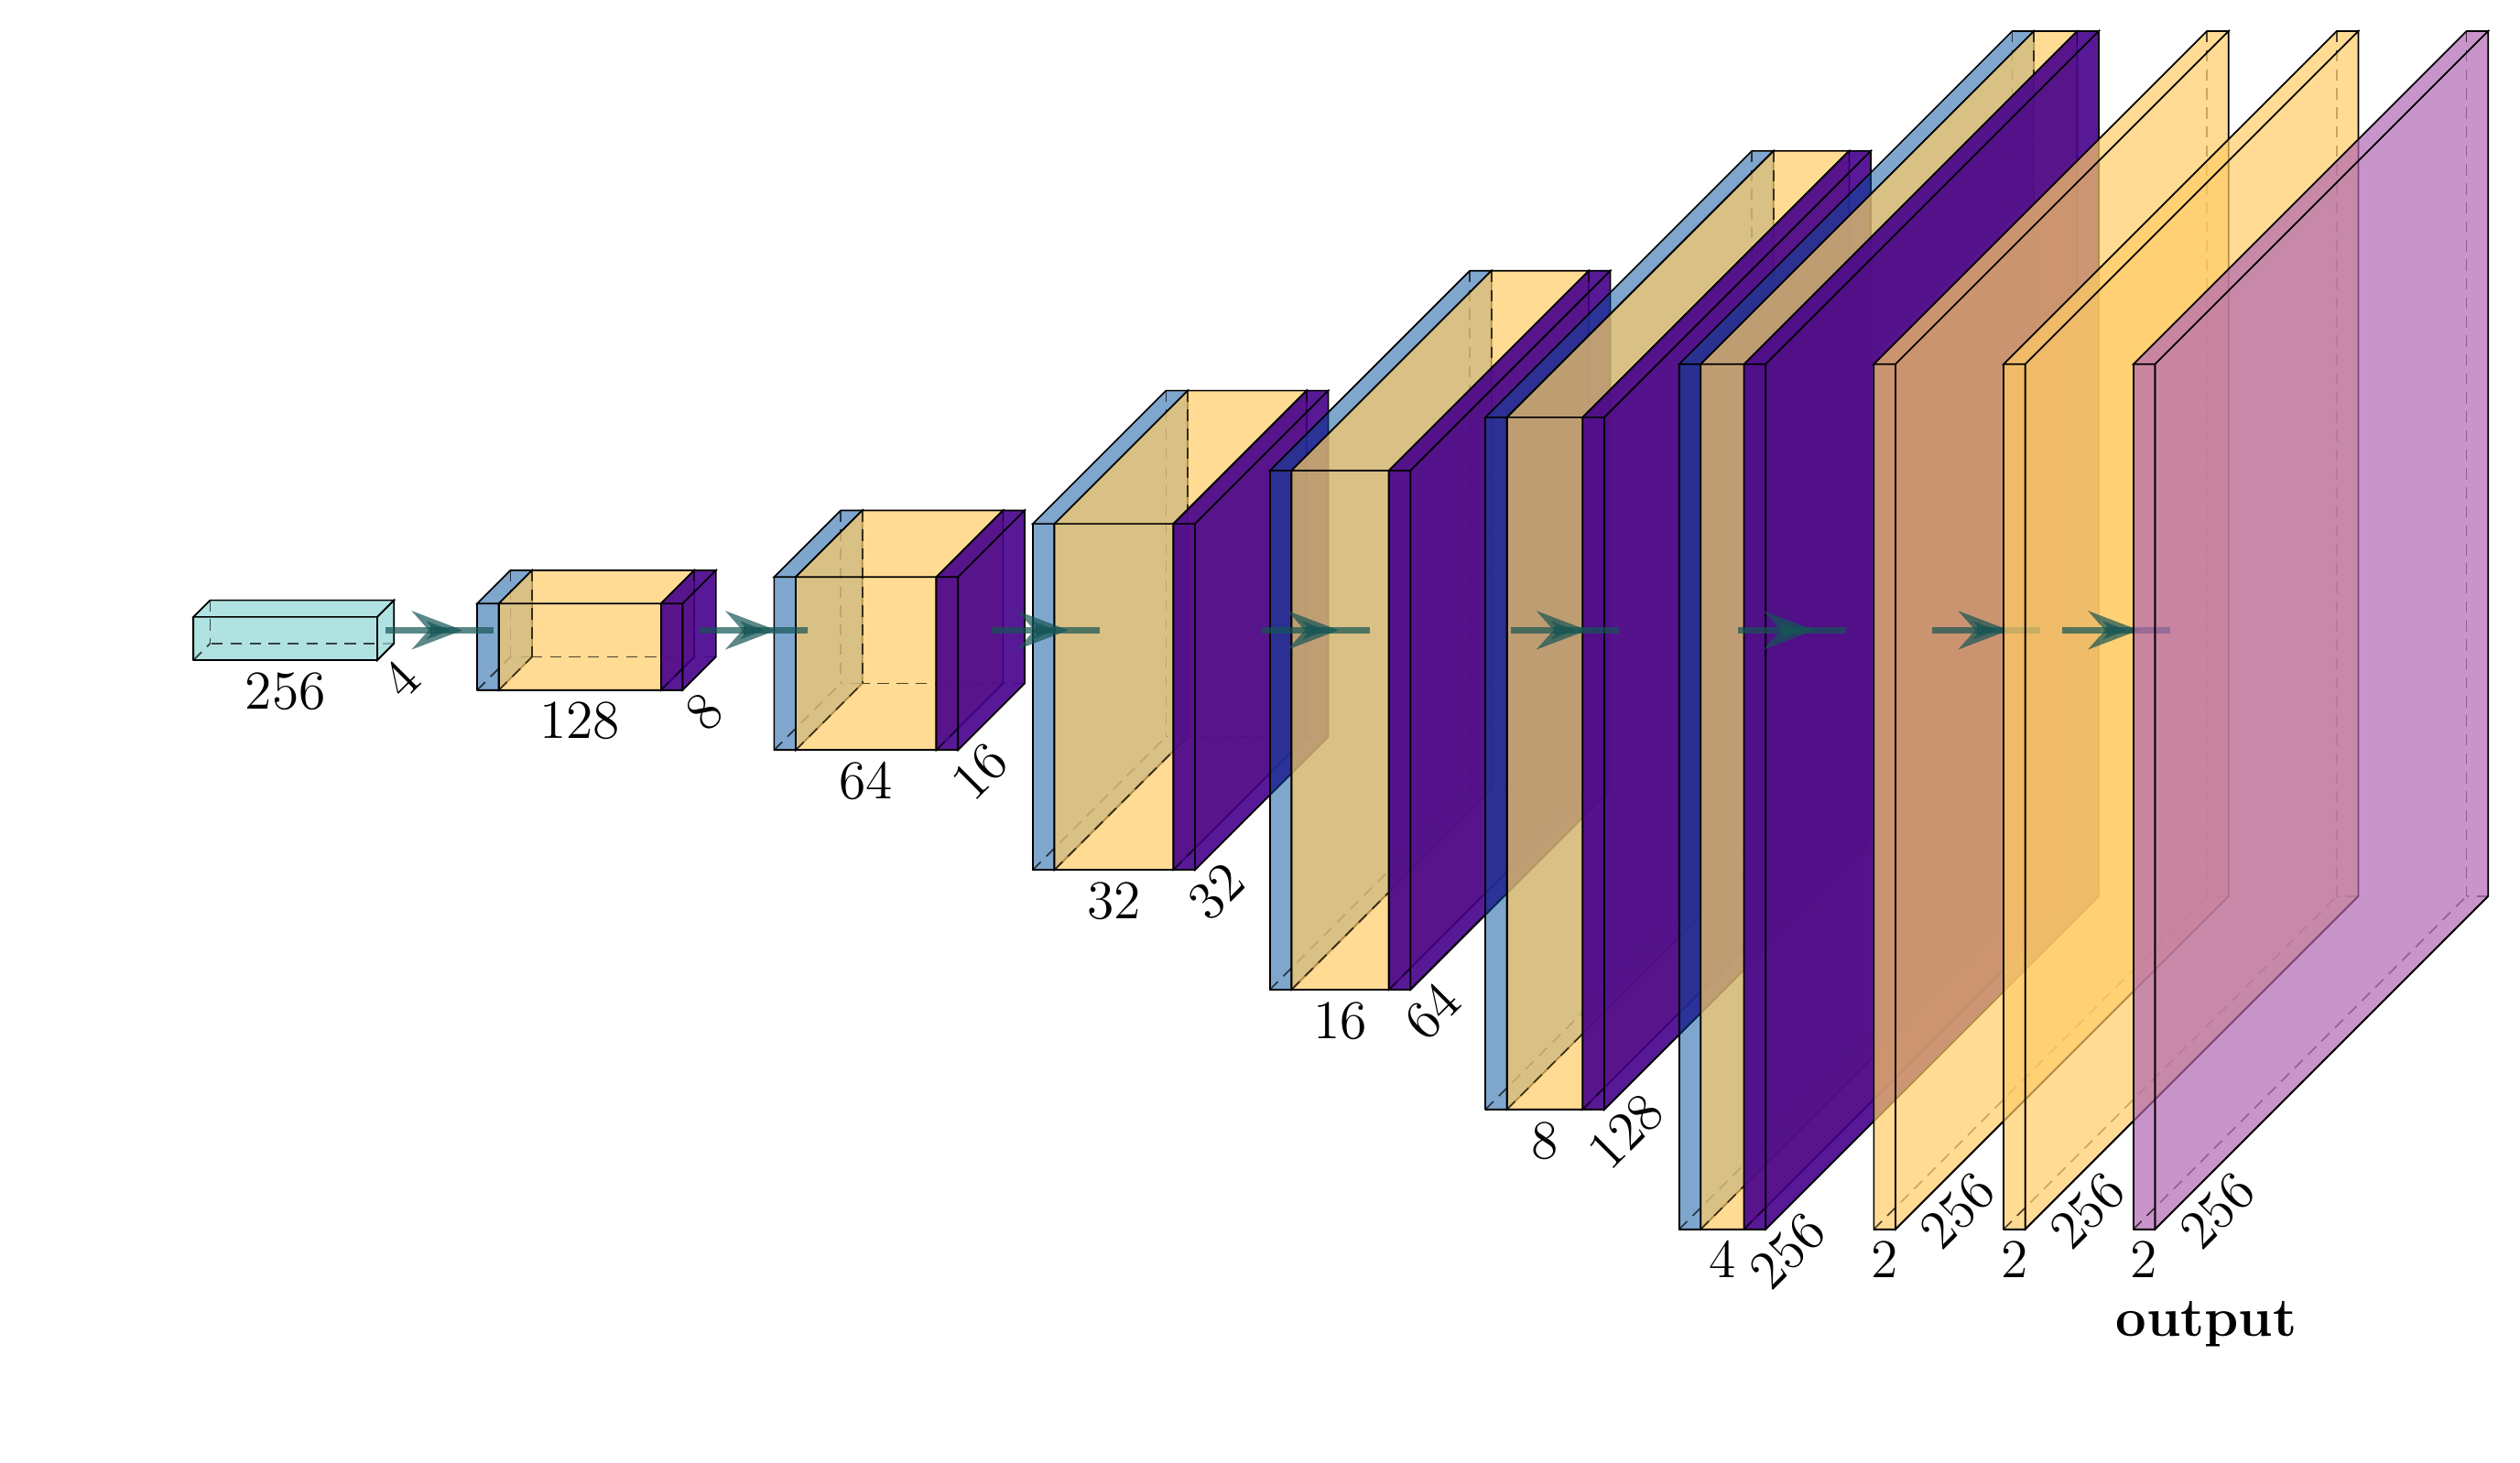
\includegraphics[width=\linewidth]{figures/Methodology/decoder.png}
    \caption{Example decoder architecture with $n_\text{conv}=6$, $p=2$, $k=3$, $C_\text{in}=4$ and $C_\text{base}=8$. \\ The colour coding for each layer is:
      upsampling: \colorbox{\UnpoolColor}{\phantom{x}},
      2D-convolution:~\colorbox{\ConvColor}{\phantom{x}},
      GELU activation: \colorbox{\GeluColor}{\phantom{x}} \& 
      compressed feature map:~\colorbox{\FeatColor}{\phantom{x}}}
    \label{fig: decoder}
\end{figure}

Batch normalisation is not included in the decoder, because the goal of the decoder is to reconstruct a specific physical field with known statistics (like divergence, kinetic energy or mean velocity), and it thus should not regularise the intermediate feature maps as it would interfere with the correct reconstruction of the learned flow states. 

The full layer-by-layer specification of the autoencoder visualised in Figure~\ref{fig: AE} is summarised in \autoref{tab: AE_params}. The dense bottleneck layers account for approximately 95\% of the total parameter count, reflecting the high dimensionality of the flattened feature maps relative to the latent space.

\begin{table}[H]
\centering
\caption{Layer-by-layer summary of the autoencoder architecture. Spatial dimensions 
refer to the feature map size after each operation. The total number of trainable 
parameters is 17\,638\,548.}
\label{tab: AE_params}
\small
\begin{tabular}{llrrr}
\toprule
\textbf{Component} & \textbf{Layer} & \textbf{Output size} & \textbf{Parameters} \\
\midrule
\multicolumn{4}{l}{\textit{Encoder}} \\
Input           &                                   & $256\times256\times4$   &           \\
Block 1         & Conv $3\times3$, ReLU, MaxPool     & $128\times128\times8$   & 296       \\
Block 2         & Conv $3\times3$, BN, ReLU, MaxPool & $64\times64\times16$    & 1\,200    \\
Block 3         & Conv $3\times3$, BN, ReLU, MaxPool & $32\times32\times32$    & 4\,704    \\
Block 4         & Conv $3\times3$, BN, ReLU, MaxPool & $16\times16\times64$    & 18\,624   \\
Block 5         & Conv $3\times3$, BN, ReLU, MaxPool & $8\times8\times128$     & 74\,112   \\
Block 6         & Conv $3\times3$, ReLU, MaxPool      & $4\times4\times256$     & 295\,168  \\
Flatten         &                                   & $4096$                  &           \\
Dense 1         & Linear, ReLU                      & $2048$                  & 8\,390\,656 \\
Dense 2         & Linear                            & $16$                    & 32\,784   \\
\midrule
\multicolumn{4}{l}{\textit{Latent space $\mathbf{z} \in \mathbb{R}^{16}$}} \\
\midrule
\multicolumn{4}{l}{\textit{Decoder}} \\
Dense 3         & Linear, ReLU                      & $2048$                  & 34\,816   \\
Dense 4         & Linear, Reshape                   & $4\times4\times256$     & 8\,392\,704 \\
Block 7         & Upsample, Conv $3\times3$, GELU   & $8\times8\times128$     & 295\,040  \\
Block 8         & Upsample, Conv $3\times3$, GELU   & $16\times16\times64$    & 73\,792   \\
Block 9         & Upsample, Conv $3\times3$, GELU   & $32\times32\times32$    & 18\,464   \\
Block 10        & Upsample, Conv $3\times3$, GELU   & $64\times64\times16$    & 4\,624    \\
Block 11        & Upsample, Conv $3\times3$, GELU   & $128\times128\times8$   & 1\,160    \\
Block 12        & Upsample, Conv $3\times3$, GELU   & $256\times256\times4$   & 292       \\
Projection      & Conv $3\times3$                   & $256\times256\times2$   & 74        \\
Smoothing       & Conv $3\times3$                   & $256\times256\times2$   & 38        \\
\midrule
\textbf{Total}  &                                   &                         & \textbf{17\,638\,548} \\
\bottomrule
\end{tabular}
\end{table}

\subsection{Loss Function}
\label{sect: AEloss}
Following the physics-informed surrogate models introduced in \ref{subsect: data driven ROMS}, the autoencoder in this work is trained by minimising a composite loss function \ref{eq: AE_loss} that combines a reconstruction accuracy term with two physics-based regularisers derived from the physical and numerical properties of the simulation we are aiming to enhance. 

\begin{equation}\label{eq: AE_loss}
    \mathcal{L}_\text{AE} 
    = \mathcal{L}_\text{rec} 
    + \lambda_\text{div}\,\mathcal{L}_\text{div} 
    + \lambda_\text{curl}\,\mathcal{L}_\text{curl}
\end{equation}

The reconstruction loss $\mathcal{L}_\text{AE}$ measures the pointwise accuracy of the encoded and decoded velocity field against the reference field $\mathbf{u}$ produced by WaterLily.

\begin{equation}\label{eq: rec_loss}
    \mathcal{L}_\text{rec}
    = \bigl\langle
        \bigl\| \mathbf{u} - \psi_\theta(\varphi_\theta(\mathbf{u})) \bigr\|
      \bigr\rangle
\end{equation}

Where $\|\cdot\|$ denotes a general norm like L1 or L2 over all spatial locations and velocity components, and $\langle \cdot \rangle$ denotes an average over the available data during training. The reconstruction target is the $N_u$ dimensional velocity field $\mathbf{u}$; the kernel moment $\boldsymbol{\mu_0}$ is excluded from the target since it is a static geometric field fully determined by the signed-distance function and carries no temporal dynamics that the autoencoder needs to learn.

The divergence loss $\mathcal{L}_\text{div}$ regularises the autoencoder to respect the incompressibility constraint~\ref{eq: continuity} in the reconstructed velocity field, and is computed as the mean squared divergence over the interior domain: 

\begin{equation}\label{eq: div_loss}
    \mathcal{L}_\text{div}
    = \left\langle
        \left\| \frac{\partial \hat{u}_i}{\partial x_i} \right\|_2^2
      \right\rangle
\end{equation}

Here, divergence is discretised using the same second-order central differences scheme as WaterLily's internal finite-volume scheme. Since WaterLily is an incompressible solver, we know that the divergence of the reconstructed velocity field should be equal to zero. By penalising the autoencoder for violating mass conservation, we know that the compressed latent trajectories, on which the neural ODE is trained, will contain minimal residual information that could lead to mass conservation violations. This is especially important during later inference rollouts, as these latent divergence residuals could accumulate, leading to reconstructed flow states that massively violate mass conservation.

The vorticity loss $\mathcal{L}_\text{curl}$ penalises differences between the vorticity of the reference and reconstructed velocity fields:

\begin{equation}\label{eq: curl_loss}
    \mathcal{L}_\text{curl}
    = \left\langle
        \left\| \omega - \hat{\omega} \right\|_2^2
      \right\rangle,
    \qquad
    \omega = \frac{\partial u_j}{\partial x_i} - \frac{\partial u_i}{\partial x_j}
\end{equation}

Where $\hat{\omega}$ denotes the vorticity of the reconstructed flow snapshot $\mathbf{\hat{u}}$. The inclusion of the vorticity loss serves 2 purposes. First, the vorticity $\omega$ is constructed from the off-diagonal components of the velocity gradient tensor, $\partial u_i / \partial x_j$ and $\partial u_j / \partial x_i$, which are important for shear related phenomana in the flow. Without imposing an explicit penalty on these off-diagonal derivatives, the autoencoder can struggle to accurately reconstruct the sharp gradients that define the shed vortices and the boundary-layer separation near the cylinder surface. Secondly, the Biot-Savart boundary conditions rely on the fluid's vorticity to determine the velocity at the domain boundary. By training the autoencoder to accurately reconstruct the vorticity of a flow snapshot, the decoded velocity fields are more likely to produce boundary-consistent ghost-cell values when the Biot-Savart conditions are re-applied during the hybrid solver workflow described in \autoref{sect: coupling}. \todo{mss later reference fixing}

The weights $\lambda_\text{div}$ and $\lambda_\text{curl}$ are tunable hyperparameters that control the relative importance of each physics constraint during training. Setting them too low could allow the autoencoder to minimise the reconstruction loss without respecting the flow's physics. Setting them too high biases the optimiser toward the physics terms, potentially degrading pointwise accuracy. The choice of these weights thus involves a balance: they should be large enough to regularise the latent trajectories and produce physically relevant reconstructions, but not so large that they dominate the loss landscape and prevent the reconstruction term from driving the network to learn finer-scale flow features.  



\subsection{Training Setup}
\label{sect: AEtraining}

% Since the framework in this thesis is designed to run in line with a running WaterLily simulation, the autoencoder is trained on a range of snapshots from the same simulation. Where the gathered snapshots are split temporally first, according to the preset run time of the simulation $t_\text{run}$, then all snapshots with $t^* < t^*_\text{train}$ form the training and validation pool, from which $N_\text{train}$ snapshots are sampled at uniform temporal spacing; an additional $20\%$ of these are held out as a validation set for epoch-level monitoring. The remaining snapshots are drawn exclusively from $t_\text{run} > t^* \geq t^*_\text{train}$, and form a held-out test set used to assess generalisation beyond the training horizon. 


Since the framework in this thesis is designed to run in line with a running WaterLily simulation, the autoencoder is trained on a range of snapshots from that simulation. Where the gathered snapshots are split temporally first, according to the preset run time of the simulation $t_\text{run}$, then all snapshots with $t^* < t^*_\text{train}$ form the training and validation pool. A temporal split was chosen over a random split because the latter would have allowed snapshots that are separated by less than a fraction of a shedding period to be assigned to different splits; given the strong periodicity of the flow, such near-duplicate pairs would cause the validation and test errors to collapse onto the training error and limit any proper analysis of the loss of generalisation beyond the training horizon. From the training and validation pool, $N_\text{train}$ snapshots are sampled at uniform temporal spacing, of which an additional $20\%$ are held out as a validation set for epoch-level monitoring. The remaining snapshots are drawn exclusively from $t^*_\text{train} \leq t^* < t_\text{run}$, and form a held-out test set used to assess generalisation beyond the training horizon. The absolute number of snapshots in the training can be kept modest because the relevant metric of dataset quality is not the number of snapshots, but rather the number of distinct phases of the shedding cycle covered, the training window in figure~\ref{fig: train_force_split} shows how $t^*_\text{train}$ was set to include 4 main shedding cycles to ensure that sufficient temporal and spatial scales are present in the training data. 


\begin{figure}[H]
    \centering
    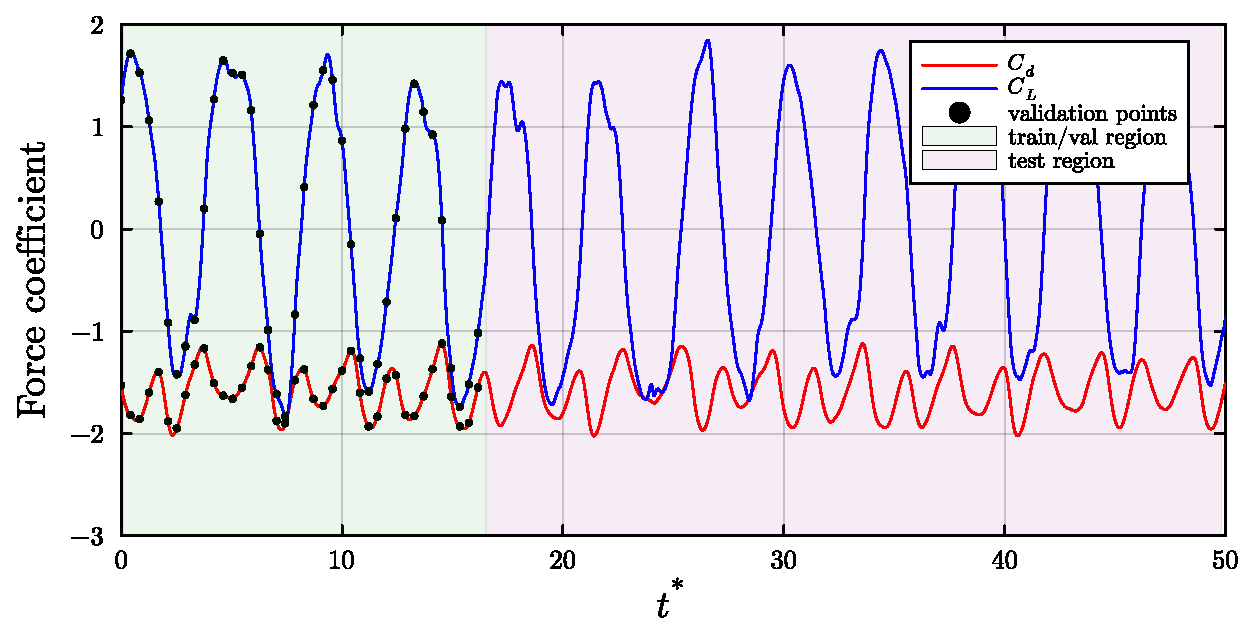
\includegraphics[width=\linewidth]{figures/Methodology/train_force_split.pdf}
    \caption{}
    \label{fig: train_force_split}
\end{figure}




During training, the network weights $\theta$ are optimised using AdamW~\cite{Loshchilov2019}. Important to note is that the encoder and decoder are optimised at the same time and thus share the same network weights, only after training is finished are the encoder and decoder treated as seperate transformations. The learning rate is set according to the training regime, be it initial training or transfer learning training, with a decoupled weight decay of $\lambda = 9 \cdot 10^{-4}$, and gradients are computed via reverse-mode automatic differentiation using \texttt{Zygote.jl}. Mini-batches of $16$ snapshots are used to ensure smooth convergence of the loss function, and to save memory on the GPU. All tensors are stored in single precision (\texttt{Float32}) and training is performed on a single NVIDIA GPU on the DelftBlue HPC cluster \cite{DHPC2024}. 


% To ensure reproducibility, all random number generators are seeded with a fixed value ($\text{seed} = 42$), and the full hyperparameter configuration is serialised alongside the network parameters and the per-channel normalisation statistics into a single \texttt{JLD2} checkpoint at the end of training. The same checkpoint is later reloaded for inference and for the transfer-learning stages described in Section~\ref{sect: AEvalidation}.


% Optimizer: Adam, η = 1e-3, weight decay λ = 9e-4.
% Batch size: 16; epochs: 1000; validation split: 20\%.
% Hardware: GPU (CUDA); precision: Float32.
% Checkpointing and early stopping strategy.

\subsection{Validation}
\label{sect: AEvalidation}

% Reconstruction error on held-out snapshots.
% Visual comparison of original vs.\ reconstructed flow fields.
% Divergence and curl residuals of reconstructed fields.
% Validate against published AE results in the literature.

% -----------------------------------------------------------------------
\section{Neural ODE}
\label{sect: NODE}

After having trained the autoencoder, each instantaneous flow field can be compressed to the low-dimensional latent space: $\mathbf{z} = \varphi_\theta(\mathbf{x}_\text{in}) \in \mathbb{R}^{N_z}$. Compressing each available snapshot in the training set in time-ordered fashion at a fixed discrete time interval $\Delta t$ (i.e., $ \mathcal{T}_{z,i} = \varphi_\theta(\mathcal{T}_{u,i}$, where $\mathcal{T}_{u,i}$ is a trajectory of full-order states) produces a sequence of latent vectors that serves as the ground truth on which the neural ODE can be trained: 


\begin{equation}\label{eq: latent_traj}
    \mathcal{T}_{z,i} = [\mathbf{z}(t_{0,i}),\, \mathbf{z}(t_{0,i} + \Delta t),\, \mathbf{z}(t_{0,i} + 2\Delta t),\, \ldots,\, \mathbf{z}(t_{0,i} + n_{t,i}\Delta t)], \quad i = 1, \ldots, N_T, \quad t_{\text{train}, i} = n_{t,i}\Delta t
\end{equation}


Where $N_T$ represents the total number of ground truth trajectories of the same system, $n_{t, i}$ and  $t_{0, i}$ denote the training trajectory length and the start time of a specific trajectory $i$, respectively, and $t_{\text{train},i}=n_{t,i}\,\Delta t$ is the corresponding trajectory duration in physical time. An example of these resulting latent trajectories is shown in Figure~\ref{fig: latent_traj} for four representative components. The latent trajectories typically consist of one or more dominant modes, such as $z_1$ and $z_4$, which exhibit a clear period behaviour that corresponds to vortex shedding frequency visible in the force history of \autoref{fig: 256_forces}. Less dominant modes such as $z_4$ and $z_{12}$ carry lower amplitudes and contain more complex frequency content that correspond to secondary vortex structures and irregular frequencies visible in figures \ref{fig: vortex_shedding} and \ref{fig: 256_forces} respectively. 


\begin{figure}[H]
    \centering
    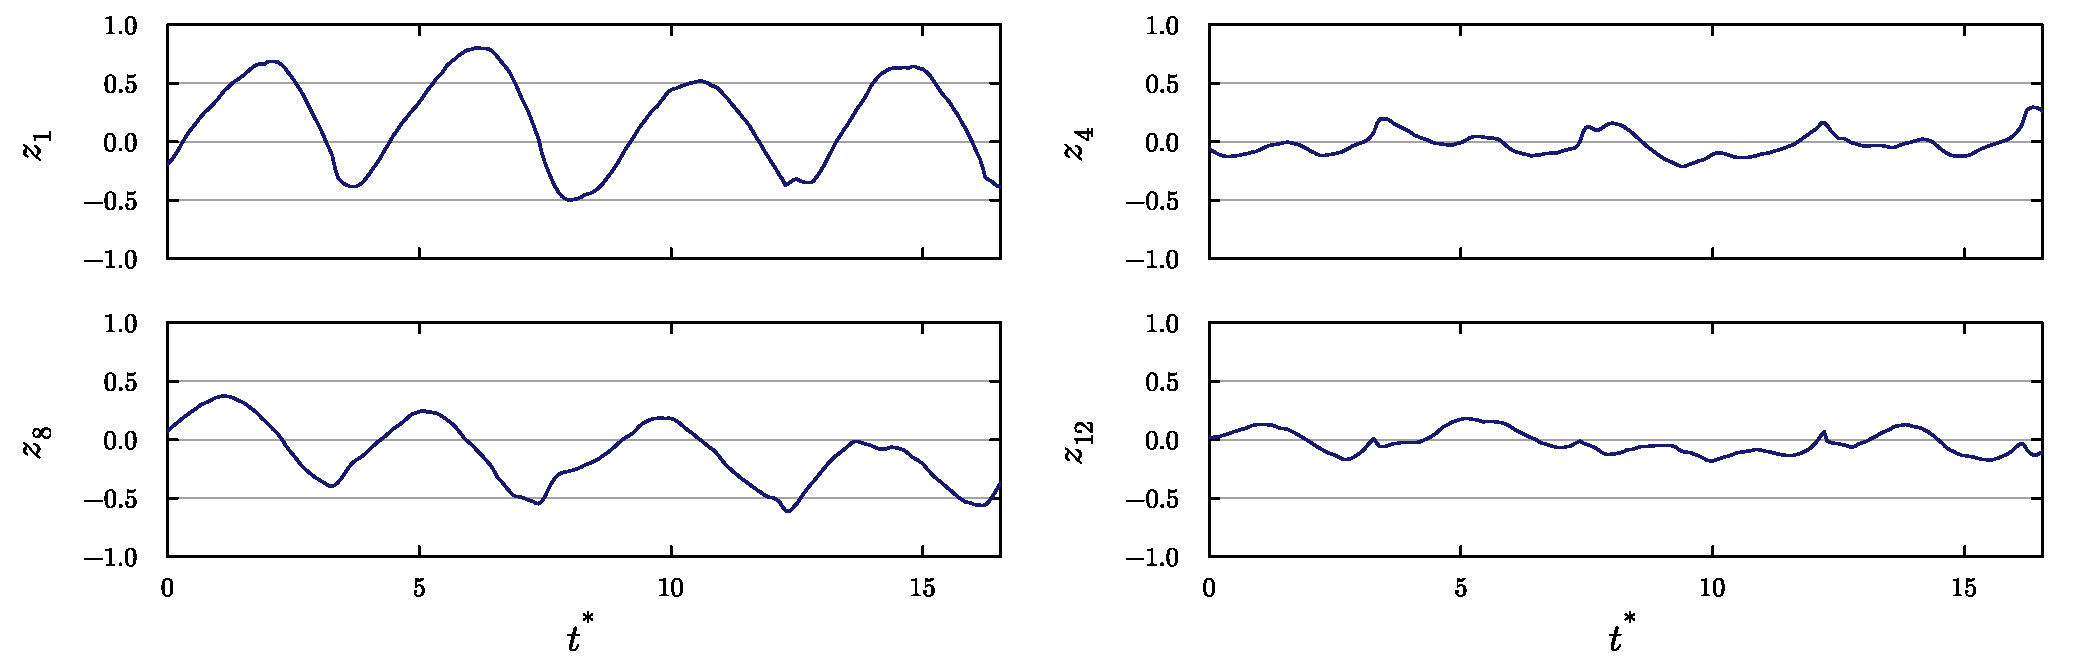
\includegraphics[width=\textwidth]{figures/Methodology/latent_trajectories.pdf}
    \caption{Representative latent components of the encoded training data over 4 shedding periods at $\mathrm{Re}=2500$. The quasi-periodic structure reflects the vortex shedding cycle captured by the autoencoder.}
    \label{fig: latent_traj}
\end{figure}

The neural ODE is tasked with learning the dynamics of this trajectory so it can integrate it forward in time. As introduced in \label{subsubsect: NODEs}, the Neural ODE parametrises the time derivative of the latent state with a neural network, so that future latent states are obtained by integrating \ref{eq: latent_NODE} from a known initial condition ($\mathbf{z}(t_{0, i})$) with a standard ODE solver

\begin{equation}\label{eq: latent_NODE}
    \frac{d\mathbf{z}(t)}{dt} = f_\phi(\mathbf{z}(t)), \qquad \mathbf{z}(t_0) = \varphi_\theta(\mathbf{x}_\text{in}(t_0)).
\end{equation}

In \ref{eq: latent_NODE} $f_\phi$ is a neural network with trainable parameters $\phi$. Given an initial condition $\mathbf{z}(t_0)$, a conventional time integrator can be used to find the latent state $\tilde{\mathbf{z}}(t)$ at any desired time $t$. This means that, for the neural ode defined above, a predicted latent trajectory can be produced that is analogous to the ground-truth trajectory in \ref{eq: latent_traj} and starts at the same initial condition \cite{Nair2024}. 

\begin{equation}\label{eq: latent_traj_pred}
    \tilde{\mathcal{T}}_{z,i} = [\tilde{\mathbf{z}}(t_{0,i}),\, \tilde{\mathbf{z}}(t_{0,i} + \Delta t),\, \tilde{\mathbf{z}}(t_{0,i} + 2\Delta t),\, \ldots,\, \tilde{\mathbf{z}}(t_{0,i} + n_{t,i}\Delta t)], \quad i = 1, \ldots, N_T,
\end{equation}

Because $N_z \ll N_x N_y N_u$, the time integration operates on a low-dimensional ODE rather than the original discretised Navier-Stokes system, making both training and inference computationally inexpensive. The following subsections highlight the architecture of $f_\phi$, the multiple-shooting training strategy used to stabilise learning over long trajectories, and the validation procedure applied to the resulting latent dynamics model.


\subsection{Architecture}
\label{sect: NODEarch}

The right-hand side of \autoref{eq: latent_NODE} is parametrised by the fully-connected neural network $f_\theta$. This MLP is deliberately kept compact, since the autoencoder has already distilled the flow states into a low-dimensional representation; a small network suffices to learn the latent dynamics. This has the added benefit of having a low computational cost during both training and time integration. A schematic of the network architecture is shown in \autoref{fig: NODE_arch}.

 \begin{figure}[H]
    \centering
    \begin{tikzpicture}[
    neuron/.style={circle, fill=black, minimum size=6pt, inner sep=0pt},
    >=stealth
]

% --- Parameters ---
\def\layersep{1.8}
\def\neuronspacing{0.35}
\def\inspacing{0.4}

% Number of neurons per layer
\def\nInput{6}
\def\nHiddenA{11}
\def\nHiddenB{11}
\def\nOutput{6}

% X positions of layers
\def\xInput{0}
\def\xHiddenA{1.8}
\def\xHiddenB{3.6}
\def\xOutput{5.4}


% Input layer
\foreach \i in {1,...,\nInput} {
    \pgfmathsetmacro{\ypos}{(\nInput-1)*\neuronspacing/2 - (\i-1)*\neuronspacing}
    \node[neuron] (I-\i) at (\xInput, \ypos) {};
}

% Hidden layer A
\foreach \i in {1,...,\nHiddenA} {
    \pgfmathsetmacro{\ypos}{(\nHiddenA-1)*\neuronspacing/2 - (\i-1)*\neuronspacing}
    \node[neuron] (HA-\i) at (\xHiddenA, \ypos) {};
}

% Hidden layer B
\foreach \i in {1,...,\nHiddenB} {
    \pgfmathsetmacro{\ypos}{(\nHiddenB-1)*\neuronspacing/2 - (\i-1)*\neuronspacing}
    \node[neuron] (HB-\i) at (\xHiddenB, \ypos) {};
}

% Output layer
\foreach \i in {1,...,\nOutput} {
    \pgfmathsetmacro{\ypos}{(\nOutput-1)*\neuronspacing/2 - (\i-1)*\neuronspacing}
    \node[neuron] (O-\i) at (\xOutput, \ypos) {};
}

% --- Draw connections ---
% Input -> Hidden A
\foreach \i in {1,...,\nInput} {
    \foreach \j in {1,...,\nHiddenA} {
        \draw[gray!50, thin] (I-\i) -- (HA-\j);
    }
}

\draw[thick, dotted] (HA-6.east) -- (HB-6.west);

% Hidden B -> Output
\foreach \i in {1,...,\nHiddenB} {
    \foreach \j in {1,...,\nOutput} {
        \draw[gray!50, thin] (HB-\i) -- (O-\j);
    }
}

% --- Bounding box ---
\draw[thick, rounded corners=3pt]
    ([xshift=-0.4cm, yshift=1.1cm] I-1.north west)
    rectangle
    ([xshift=0.4cm, yshift=-1.1cm] O-\nOutput.south east);

% --- Labels ---

% (a) label
% \node[anchor=north west, font=\bfseries]
    % at ([xshift=-0.25cm, yshift=0.35cm] I-1.north west) {(a)};

% Input label: \tilde{w}(t)
\node[anchor=east, font=\large]
    at ([xshift=-0.7cm] I-3.west) {$\mathbf{z}(t)$};

% Output label: d\tilde{w}(t)/dt
\node[anchor=west, font=\large]
    at ([xshift=0.7cm] O-3.east) {$\dfrac{d\mathbf{z}(t)}{dt}$};

% Network label below
\node[draw, thick, rounded corners=2pt, font=\large,
      anchor=north, inner sep=6pt]
    at ([yshift=-1.5cm] {barycentric cs:I-\nInput=1,O-\nOutput=1})
    {$f_\phi(\mathbf{z}(t))$};

% --- Arrows from box to network label ---
\pgfmathsetmacro{\bottomY}{(\nInput-1.1)*\neuronspacing/2 - (\nInput-1)*\neuronspacing - 1.1}

% Connections from bottom of bounding box to the label box
\coordinate (boxBottom) at (2.7, \bottomY - 0.05);
\coordinate (labelTop) at (2.7, \bottomY - 0.4);

\draw[thick] (boxBottom) -- (labelTop);

\end{tikzpicture}
    \caption{Architecture of the Neural ODE right-hand side $f_\phi(\mathbf{z})$}
    \label{fig: NODE_arch}
\end{figure}

\todo{nog iets over activation function schrijven}

Given an initial condition $\mathbf{z}(t_0) = \varphi_\theta(\mathbf{x}_\text{in}(t_0))$, future latent states are obtained by numerically integrating \autoref{eq: latent_NODE} with a common numerical ODE solver like the Tsitouras 5th-order Runge--Kutta method (\texttt{Tsit5}). 

% ODE function: fully-connected network latent_dim → (dense_mult × latent_dim) → latent_dim.
% dense_mult = 3, activation = tanhshrink.
% Justify depth, width, and activation function choice.

% \subsection{ODE Solver}
% \label{sect: solver}

% Tsit5 adaptive solver; reltol = 1e-4, abstol = 1e-6.
% Justify choice of adaptive solver for stiff-free latent dynamics.

\subsection{Training with Multiple Shooting}
\label{sect: NODEtraining}

The parameters $\phi$ of the feed-forward network $f_\phi$ in the neural ODE are typically optimised by minimising an objective function, like the mean squared error, between the ground truth trajectories $\mathcal{T}_{z,i}$ and the predicted trajectories $\tilde{\mathcal{T}}_{z,i}$ during the training stage using a standard optimiser like \texttt{AdamW}. This objective function would then be given by:

\begin{equation}\label{eq: node_loss_naive}
    \mathcal{L}_{\text{NODE}} = \left\langle \frac{1}{n_{t}} \sum_{j=1}^{n_{t}} \left\| \mathbf{z}(t_{0} + j\Delta t) - \tilde{\mathbf{z}}(t_{0} + j\Delta t) \right\|_2^2 \right\rangle
\end{equation}

Where $\langle \cdot \rangle$ denotes the average over all available training trajectories $N_T$ and the inner sum accumulates the per-snapshot reconstruction error. Training the neural ODE by directly minimising~\eqref{eq: node_loss_naive} requires integrating the full latent trajectory from a single initial condition $\tilde{\mathbf{z}}(t_{0,i})$ and back-propagating through the entire rollout is conceptually the simplest approach. It fails reliably over longer rollouts required to capture a sufficient number of shedding cycles in the regime considered here.

This approach, called single shooting, fails because the optimiser must simultaneously select parameters $\phi$ that fit the predicted trajectory to every snapshot along its full length~\cite{Turan2022}. For oscillatory problems or long rollouts, this is a difficult optimisation problem with many local minima. Additionally, neural networks exhibit a spectral bias during gradient descent training, leading to the fact that low-frequency components of the target function are learned more easily than high-frequency ones \cite{Rahaman2019}. 

\begin{figure}[H]
    \centering
    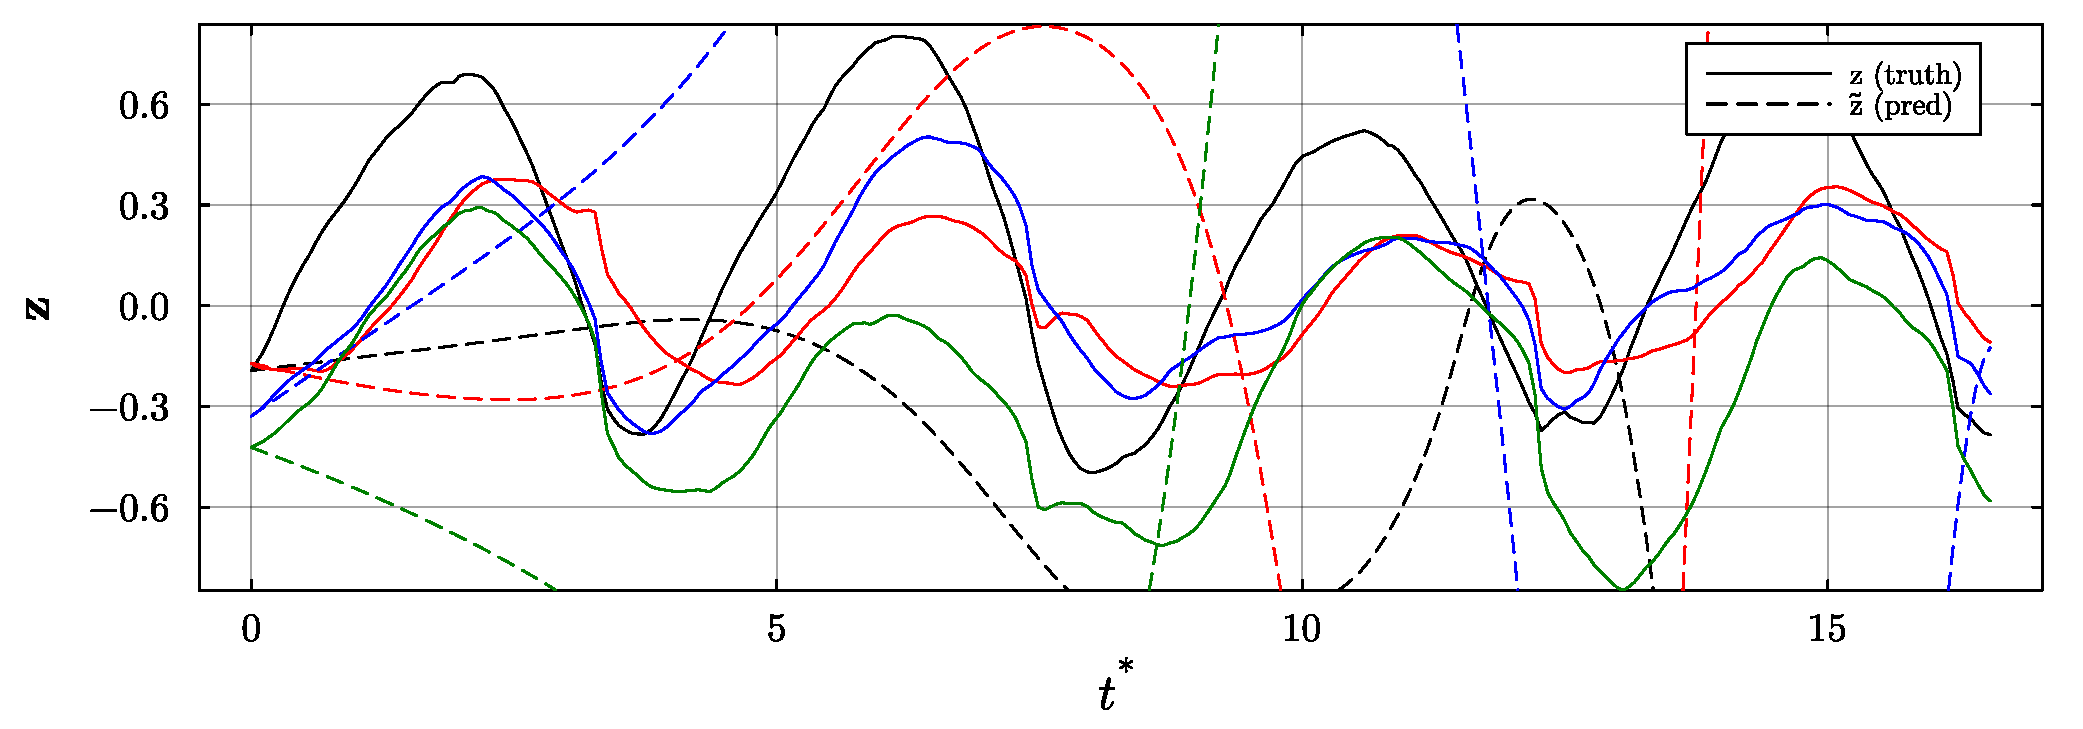
\includegraphics[width=\linewidth]{figures/Methodology/trajectories.pdf}
    \caption{Single-shooting training of the neural ODE on a representative latent trajectory at $\mathrm{Re} = 2500$, displaying 4 latent components. Illustrating the failure mode single-shooting suffers from during long rollouts}
    \label{fig: singleshoot}
\end{figure}

Figure~\ref{fig: singleshoot} shows how the learned latent trajectory gets stuck learning the complex, multi-frequency latent dynamics when operating in a single-shooting fashion. 

To avoid this failure mode of the single shooting, the neural ODE is trained using \emph{multiple shooting}, a method originally developed for boundary-value problems in numerical analysis~\cite{Bock1984} and adapted to neural ODEs by~\textcite{Turan2022}. The central idea is to replace the single, long integration required by single-shooting with several short, independent integrations whose endpoints are constrained to overlap. A specific trajectory $\mathcal{T}_{z}$, spanning $[t_{0},\, t_{\text{train}}]$, is partitioned into $N_{s}+1$ shorter intervals by introducing a grid of shooting points $t_{0} = \tau_0 < \tau_1 < \dots < \tau_{N_{s}} = t_\text{train} $, where each shooting group exists of $n_s$ samples of $\mathcal{T}_z$. At each interval, the neural ODE is integrated as an independent initial-value problem, with its initial condition treated as an additional optimisation variable. Figure \ref{fig: multiple_shoot_example} shows how the trajectory $\tilde{\mathcal{T}}_{z}$ is therefore allowed to be discontinuous across interval boundaries during training, and the resulting shooting gaps. 

\begin{figure}[H]
    \centering
    

% =====================================================================
% Multiple Shooting Schematic
% =====================================================================
% Easy-to-modify parameters:
%   - shootingBlue : color of the shooting-gap markers and labels
%   - shootingNodes: list of (x0, x0_value, xf, xf_value) per segment
%   - data points  : list of (x, y) coordinates
%   - curve segs   : three smooth curves f_hat for each segment
% =====================================================================

\begin{tikzpicture}[
    % ---- Styles ----------------------------------------------------
    shootingBlue/.style = {color=blue!70!cyan},
    axisStyle/.style    = {->, >=Latex, thick, gray!70},
    curveStyle/.style   = {thick, black, smooth},
    dataDot/.style      = {circle, fill=gray!70, inner sep=0pt, minimum size=2.2pt},
    gapLine/.style      = {shootingBlue, thick},
    openCircle/.style   = {circle, draw=blue!70!cyan, fill=white,
                           line width=0.8pt, inner sep=0pt, minimum size=5pt},
    tickStyle/.style    = {gray!70},
    x=1.1cm, y=1.1cm
]

% ---------- Axes ----------------------------------------------------
\draw[axisStyle] (-0.2,0) -- (6.8,0);
\draw[axisStyle] (0,-0.2) -- (0,4.4);

% x-axis ticks and labels
% \foreach \x in {1,2,3,4,5,6} {
%     \draw[tickStyle] (\x,0) -- (\x,-0.08);
%     \node[gray!80, font=\small] at (\x,-0.3) {\x};
% }

% x-axis ticks and labels
\foreach \x in {1,2,3} {
    \draw[tickStyle] (\x*2,0) -- (\x*2,-0.08);
    \node[gray!80, font=\small] at (\x*2,-0.3) {$\tau_\text{\x}$};
}

% y-axis ticks and labels
\foreach \y in {1,2,3,4} {
    \draw[tickStyle] (0,\y) -- (-0.08,\y);
    \node[gray!80, font=\small] at (-0.3,\y) {\y};
}

% ---------- Smooth curve segments (f_hat) ---------------------------
% Segment 1: from (0, 1.2) to (2, 3.55) -- the curve passes through node at start
\draw[curveStyle]
    (0, 1.2)
    .. controls (0.3, 1.3) and (0.5, 2.3) ..
    % (0.8, 2.1)
    % .. controls (1.1, 1.95) and (1.3, 2.8) ..
    (1.6, 3.3)
    .. controls (1.8, 3.5) and (1.9, 3.55) ..
    (2, 3.55);

% Segment 2: from (2, 2.7) to (4, 3.3)
\draw[curveStyle]
    (2, 2.7)
    .. controls (2.5, 3.0) and (3.2, 3.35) ..
    (4, 3.3);

% Segment 3: from (4, 1.6) to (6, 1.1)
\draw[curveStyle]
    (4, 1.6)
    .. controls (4.6, 1.55) and (5.2, 1.05) ..
    (5.5, 1.1)
    .. controls (5.7, 1.13) and (5.85, 1.1) ..
    (6, 1.1);

% ---------- Data points (gray dots near the curve) ------------------
\foreach \pt in {
    (0.25, 1.35), (0.55, 1.7), (0.75, 2.15),
    (1.05, 1.95), (1.35, 2.55), (1.55, 3.15),
    (1.85, 3.45),
    (2.4, 2.95), (2.9, 3.15), (3.4, 3.3), (3.75, 3.35),
    (4.4, 1.5), (4.9, 1.35), (5.3, 1.2), (5.75, 1.05)
} {
    \node[dataDot] at \pt {};
}

% ---------- Shooting gaps (vertical blue lines) ---------------------
% Gap at x = 2 : between x_f^{(1)} (top) and x_0^{(2)} (bottom)
\draw[gapLine] (2, 2.7) -- (2, 3.55);
% Gap at x = 4 : between x_f^{(2)} (top) and x_0^{(3)} (bottom)
\draw[gapLine] (4, 1.6) -- (4, 3.3);

% ---------- Shooting-gap endpoints (open blue circles) --------------
% Segment 1
\node[openCircle] at (0, 1.2)  {};  % x_0^{(1)}
\node[openCircle] at (2, 3.55) {};  % x_f^{(1)}
% Segment 2
\node[openCircle] at (2, 2.7)  {};  % x_0^{(2)}
\node[openCircle] at (4, 3.3)  {};  % x_f^{(2)}
% Segment 3
\node[openCircle] at (4, 1.6)  {};  % x_0^{(3)}
\node[openCircle] at (6, 1.1)  {};  % x_f^{(3)}

% ---------- Labels for the shooting nodes ---------------------------
\node[shootingBlue, font=\small, anchor=east] at (-0.05, 1.15)
    {$\tilde{\mathbf{z}}_0^{(1)}$};

\node[shootingBlue, font=\small, anchor=south] at (2, 3.7)
    {$\tilde{\mathbf{z}}_f^{(1)}$};

\node[shootingBlue, font=\small, anchor=north] at (2, 2.55)
    {$\tilde{\mathbf{z}}_0^{(2)}$};

\node[shootingBlue, font=\small, anchor=south west] at (4.05, 3.3)
    {$\tilde{\mathbf{z}}_f^{(2)}$};

\node[shootingBlue, font=\small, anchor=north east] at (3.95, 1.5)
    {$\tilde{\mathbf{z}}_0^{(3)}$};

\node[shootingBlue, font=\small, anchor=west] at (6.1, 1.0)
    {$\tilde{\mathbf{z}}_f^{(3)}$};

% ---------- Legend (top-right corner) -------------------------------
\begin{scope}[shift={(4.9, 4.0)}]
    % shooting gap entry
    \node[openCircle] at (0.1, 0) {};
    \draw[gapLine]    (0.18, 0) -- (0.6, 0);
    \node[openCircle] at (0.68, 0) {};
    \node[anchor=west, font=\small] at (0.95, 0) {shooting gap};

    % data points entry
    \node[dataDot] at (0.4, -0.4) {};
    \node[anchor=west, font=\small] at (0.95, -0.4) {data points};

    % f_hat entry
    \draw[curveStyle] (0.1, -0.8) -- (0.7, -0.8);
    \node[anchor=west, font=\small] at (0.95, -0.8) {$\tilde{\mathbf{z}}$};
\end{scope}

\end{tikzpicture}


    \caption{Multiple shooting schematic, showing the shooting gaps that need to be minimised during training, adapted from \textcite{Turan2022}}
    \label{fig: multiple_shoot_example}
\end{figure}


The learned trajectory becomes meaningful only if the shooting gaps between the beginning and end points of each segment are minimised to zero, meaning that the following constraint needs to be satisfied: 

\begin{equation}\label{eq: shooting_constraint}
    \tilde{\mathbf{z}}^{(s)}_f - \tilde{\mathbf{z}}^{(s+1)}_0 = 0, \qquad s = 1, \dots, N_{s,i},
\end{equation}

Supervised learning of neural networks is typically performed by optimising an unconstrained problem, which is related to the constrained optimisation problem \cite{Turan2022}. A common approach is to define a proxy cost function, $\mathcal{L}_{\text{ms}}$, which has the constraints as penalty terms:

\begin{equation}\label{eq: node_loss_ms}
    \mathcal{L}_{\text{ms}}
    = \left\langle
        \sum_{s=1}^{N_{s}+1} \sum_{j=1}^{n_s}
            \left\| \mathbf{z}^{(s)}_j - \tilde{\mathbf{z}}^{(s)}_j \right\|_2^2
        \;+\; \lambda_c \sum_{s=1}^{N_{s}}
            \left\| \tilde{\mathbf{z}}^{(s)}_f - \tilde{\mathbf{z}}^{(s+1)}_0 \right\|_2^2
      \right\rangle ,
\end{equation}

The first term is a cost function similar to \ref{eq: node_loss_naive}, but instead of calculating the loss over each sample in the trajectory, this term is a per-segment fit that is summed over all segments and their $n_s$ latent vectors. The second term is the \emph{continuity penalty}, weighted by $\lambda_c$, that drives the shooting gaps in~\eqref{eq: shooting_constraint} toward zero. The continuity weight $\lambda_c$ controls the trade-off between segment-wise accuracy and global trajectory coherence. It is typically set to a large value to ensure continuity, but remains a hyperparameter that needs to be tuned, as a too-large $\lambda_c$ can cause numerical issues, while a too-small $\lambda_c$ can lead to constraint violation. 

In practice, the implementation of \textcite{Turan2022} that is available in \texttt{DiffEqFlux.jl} was used in this work, in which the shooting initial conditions $\tilde{\mathbf{z}}^{(s)}_0$ are not free variables but are pinned to the ground-truth latents $\mathbf{z}^{(s)}_0$ at every iteration.  The continuity penalty in~\eqref{eq: node_loss_ms} therefore acts between the integrated endpoint $\tilde{\mathbf{z}}^{(s)}_f$ of segment $s$ and the data initial condition $\mathbf{z}^{(s+1)}_0$ of segment $s{+}1$. Figure~\ref{fig: ms_epochs} shows how the segments are fitted to the ground truth latent trajectories. 


\begin{figure}[htbp]
    \centering
    \begin{subfigure}[t]{0.48\textwidth}
        \centering
        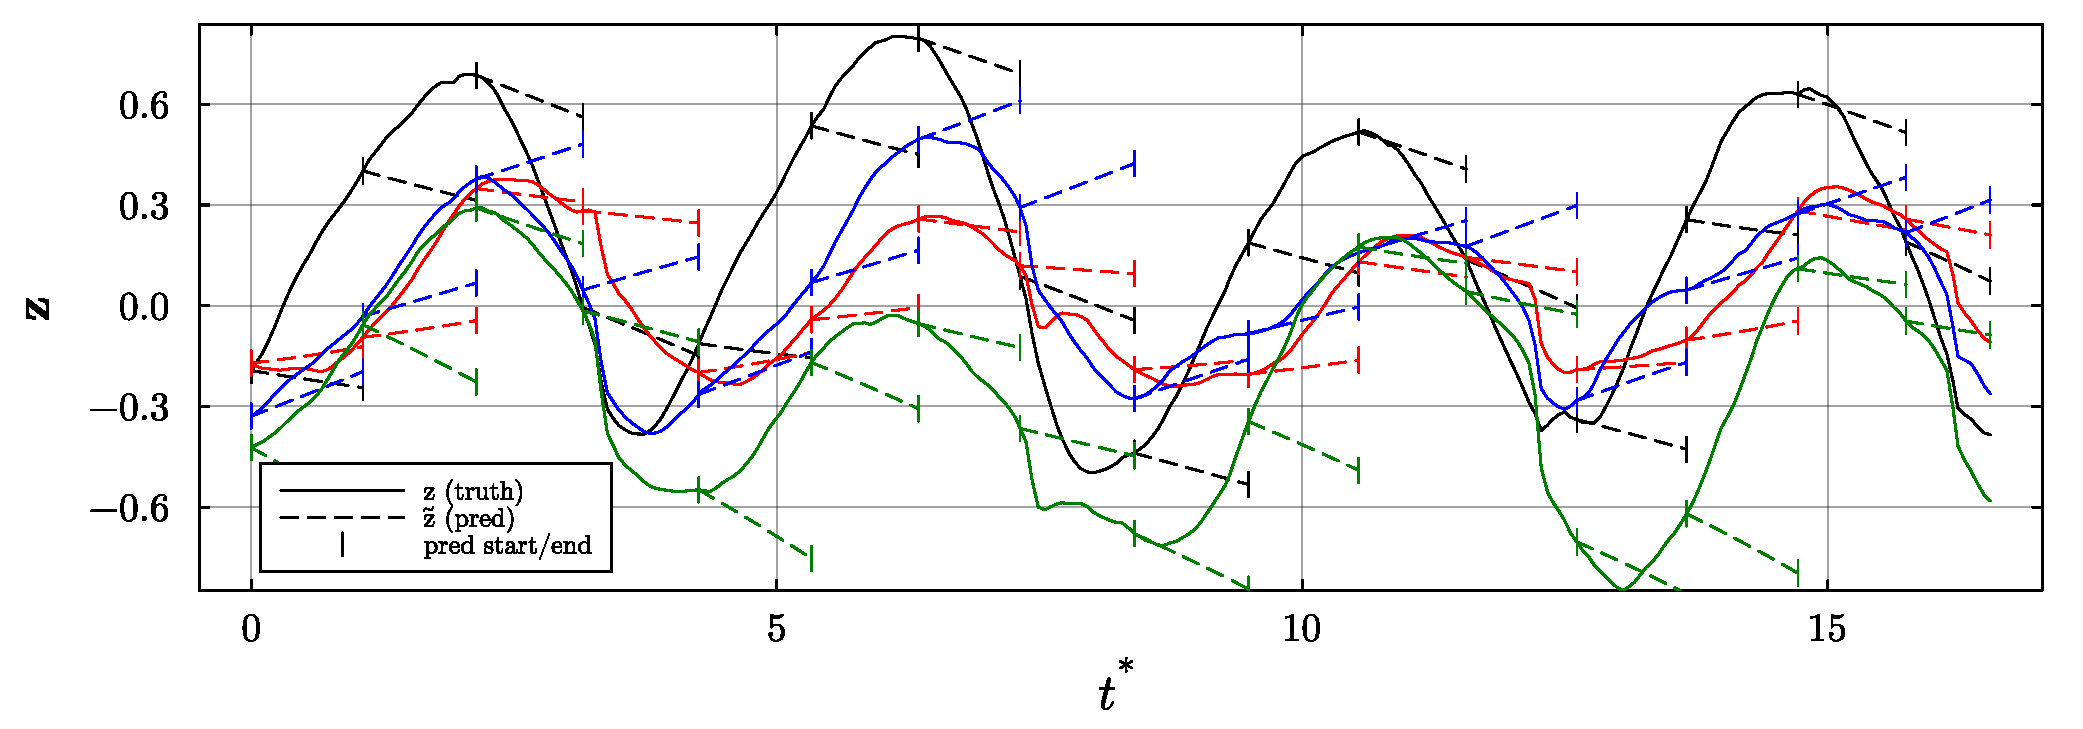
\includegraphics[width=\linewidth]{figures/Methodology/0_trajectories.pdf}
    \caption{Epoch 0: untrained network; predicted segments are nearly flat and shooting discontinuities span the full amplitude of $z$.}
    \label{fig: ms_epoch0}
    \end{subfigure}
    \hfill
    \begin{subfigure}[t]{0.48\textwidth}
        \centering
        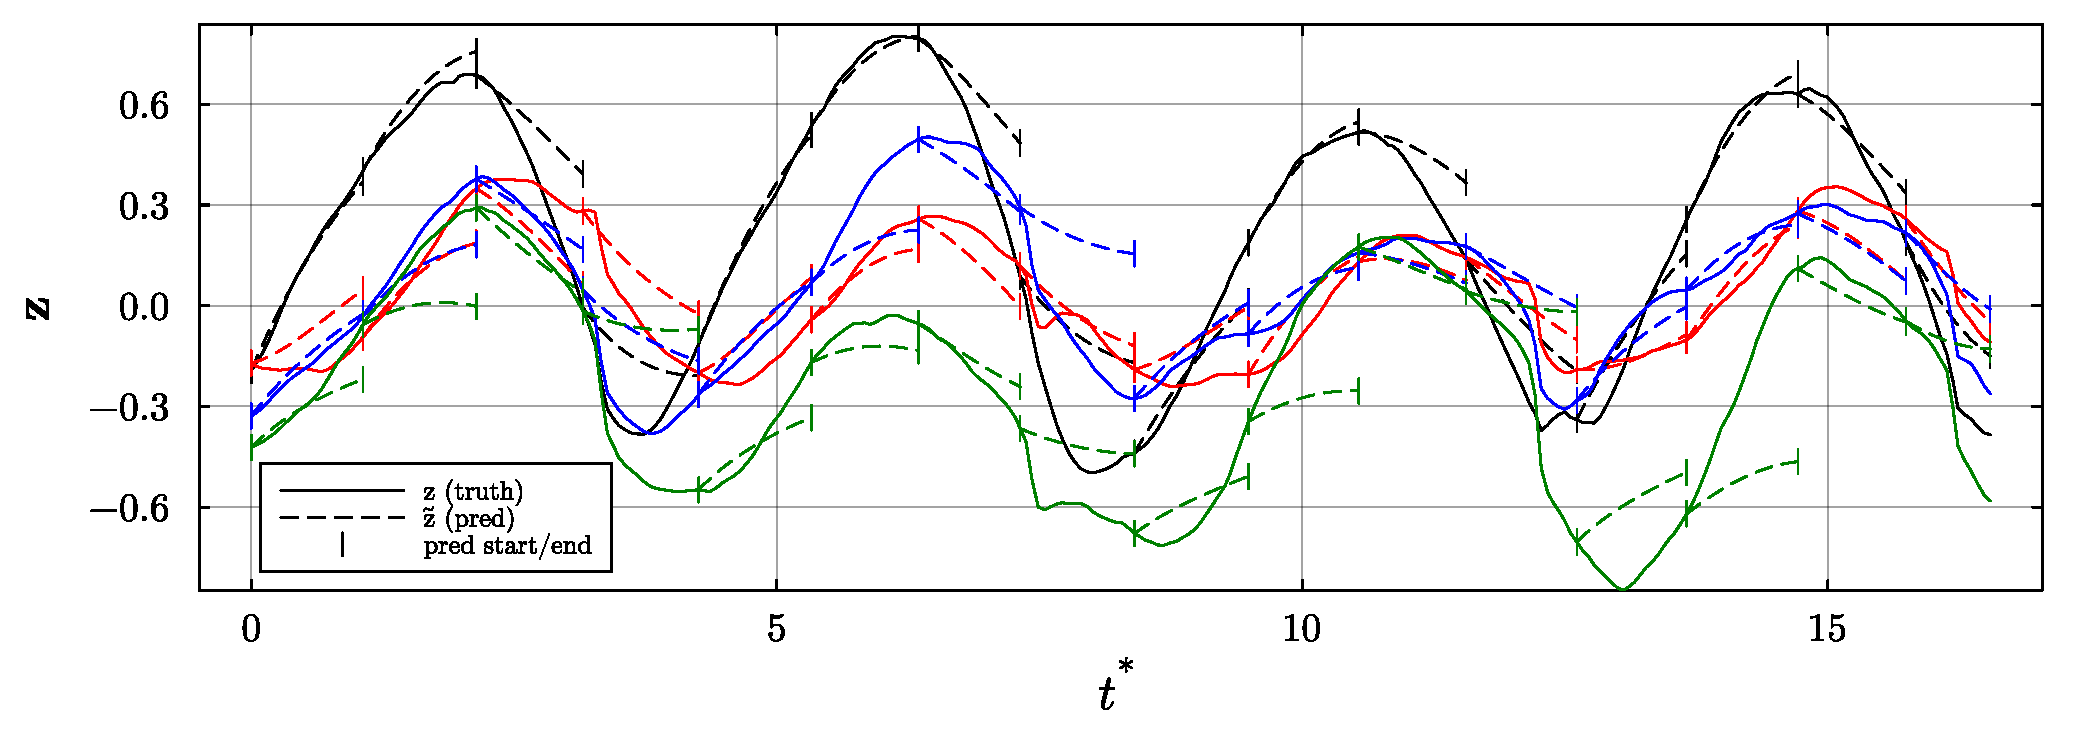
\includegraphics[width=\linewidth]{figures/Methodology/20_trajectories.pdf}
    \caption{Epoch 20: segments begin to track the reference oscillation, but visible jumps remain at every group boundary.}        
    \label{fig: ms_epoch20}
    \end{subfigure}

    \vspace{0.8em}

    \begin{subfigure}[t]{0.48\textwidth}
        \centering
        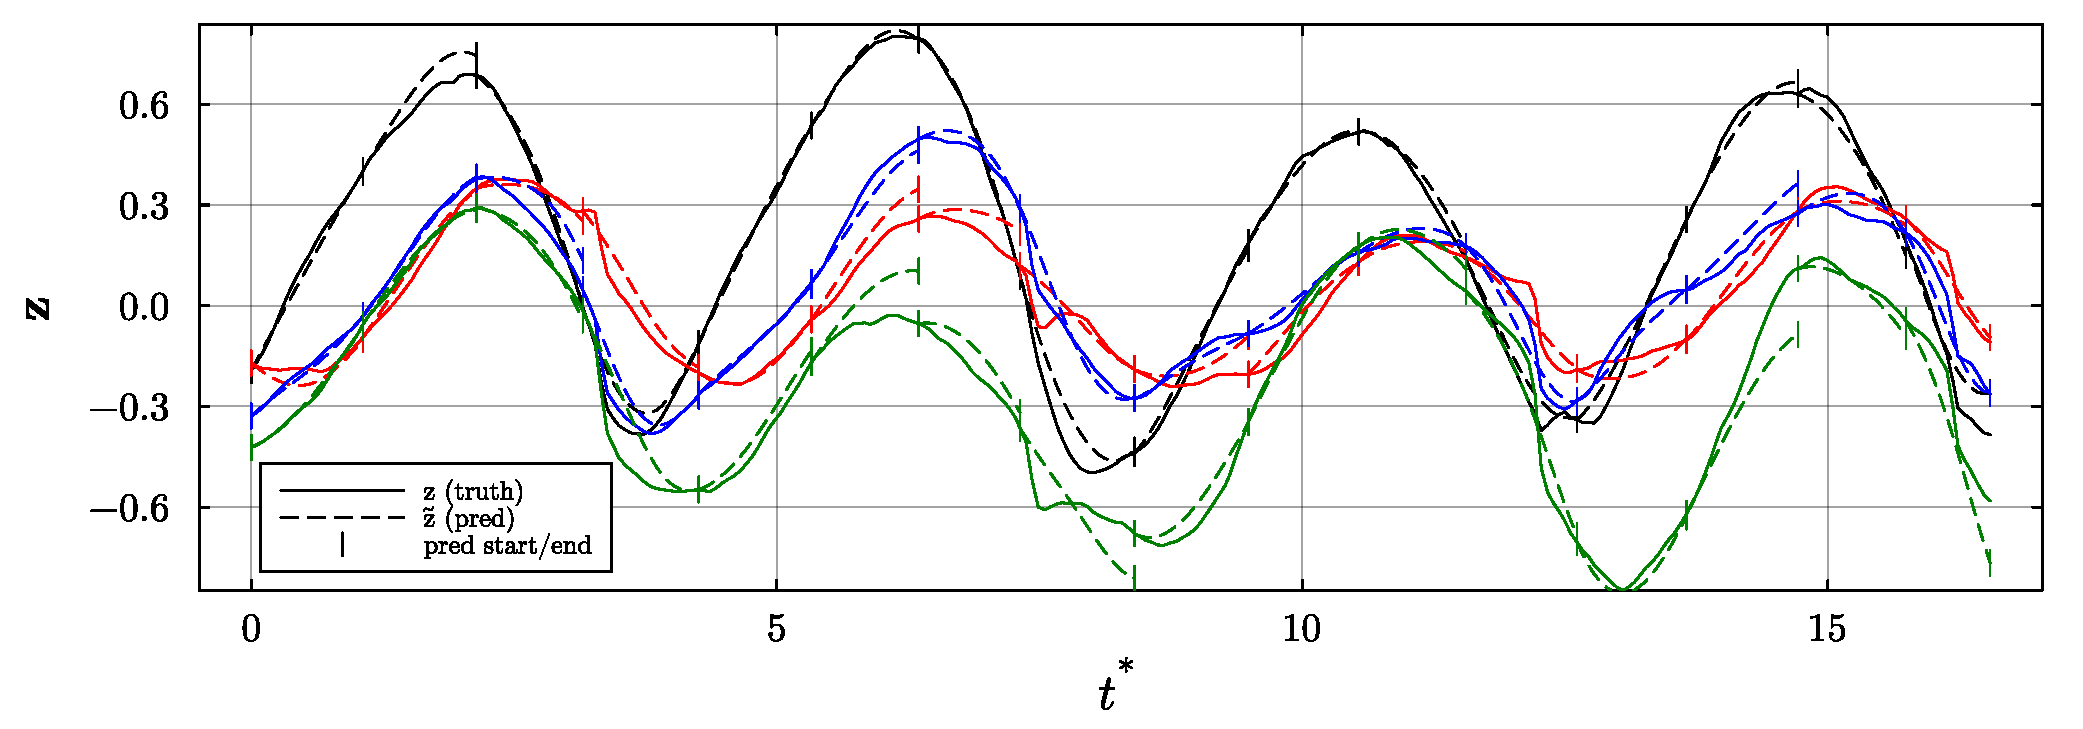
\includegraphics[width=\linewidth]{figures/Methodology/100_trajectories.pdf}
        \caption{Epoch 100: shooting discontinuities begin to close, although further refinement is still needed. }
        \label{fig: ms_epoch100}
    \end{subfigure}
    \hfill
    \begin{subfigure}[t]{0.48\textwidth}
        \centering
        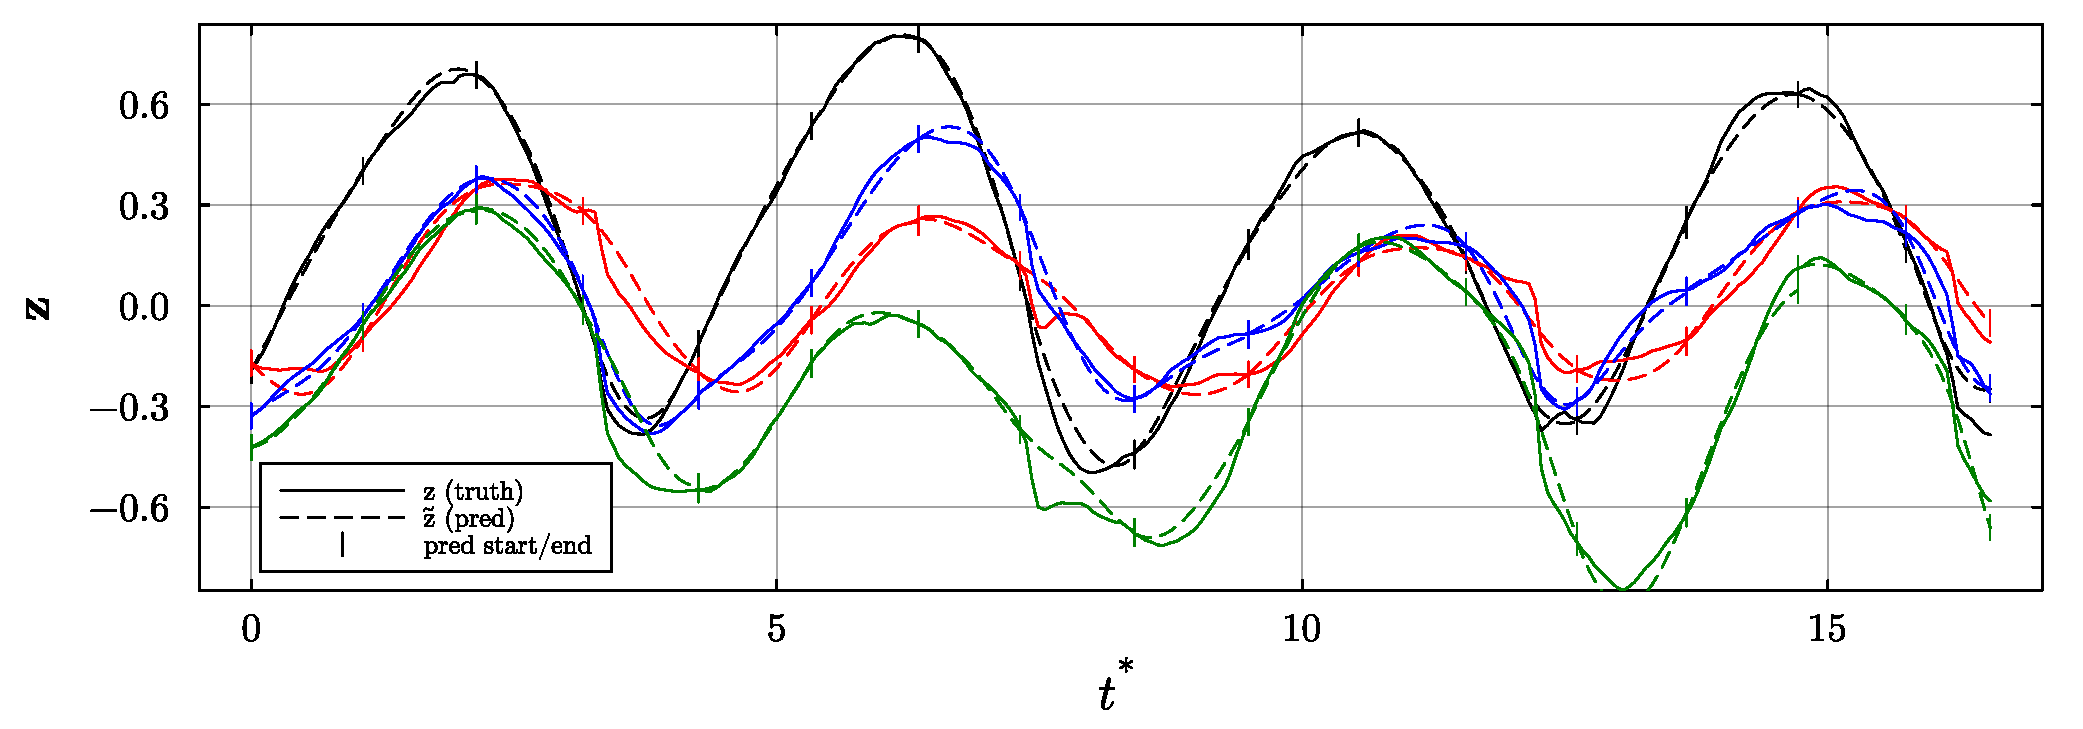
\includegraphics[width=\linewidth]{figures/Methodology/250_trajectories.pdf}
    \caption{Epoch 250: converged trajectory; predicted and reference curves overlap to within line width across the full horizon.}        
    \label{fig: ms_epoch250}
    \end{subfigure}
    \caption{Evolution of the multiple shooting latent trajectory during training. The reference trajectory $z_\mathrm{ref}$ (solid) is compared to the predicted trajectory $\tilde{z}_\mathrm{pred}$ (dashed) at four stages of training.}
    \label{fig: ms_epochs}
\end{figure}

\todo{show rollout plot over longer horizon to show drifting of NODE}


% Multiple shooting: group_size = 20, continuity_term = 200.
% Optimizer: AdamW, η = 0.01; maxiters = 250.
% Explain why multiple shooting mitigates gradient vanishing in long-horizon trajectories.
% Extrapolation flag and its role.

\subsection{Validation}
\label{sect: NODEvalidation}

\todo{begin as soon as delftblue is up and running again.}
% show influence of epochs on rollout accuracy, show influence of group size, 

% Short- and long-horizon rollout error on held-out latent trajectories.
% Comparison against trivial baselines (e.g., last-state extrapolation, linear interpolation).
% Validate latent trajectory quality against AE-encoded ground truth.

% -----------------------------------------------------------------------
\section{Out-of-Distribution Detection}
\label{sect: 3.6OOD}

% Flagging latent states that fall outside the training manifold.

\subsection{KNN-Based OOD Scoring}
\label{sect: KNN}

% KNN detector fitted on training latent vectors; distance threshold set at quantile q = 0.99 (k = 5 neighbours).
% How the score is computed at inference time and what triggers an OOD flag.

\subsection{Fallback Strategy}
\label{sect: fallback}

% When an OOD flag is raised, control is handed back to the conventional CFD solver.
% Discuss the trade-off between acceleration and safety.

% -----------------------------------------------------------------------
\section{Integrated Acceleration Workflow}
\label{sect: workflow}

% Putting the trained components together as a drop-in CFD accelerator.

\subsection{Fixed-Horizon Prediction}
\label{sect: fixedhorizon}

% \texttt{predict\_n}: encode current field → NODE integrate $n_t$ steps → decode → insert into solver.
% Describe the non-dimensionalization of the time axis (division by characteristic length = 32).

\subsection{Flexible-Horizon Prediction}
\label{sect: flexhorizon}

% \texttt{predict\_flex}: OOD-gated variant that decides how many steps to skip adaptively based on the OOD score.

\subsection{Coupling with the CFD Solver}
\label{sect: coupling}

% How predictions are inserted back into the simulation: velocity field update, pressure reset, CFL-based Δt update.
% Optional Biot boundary condition imposition after insertion.

% -----------------------------------------------------------------------
\section{Evaluation Design}
\label{sect: evaluation}

% Define all experiments to ensure results in \autoref{chap: 4} are unambiguous and reproducible.

\subsection{Accuracy Metrics}
\label{sect: accuracy}

% Field-level: mean absolute error, RMSE on velocity components.
% Trajectory: rollout divergence over time, phase drift.
% Physics consistency: divergence-free residual, force coefficient comparison.

\subsection{Speedup Metrics}
\label{sect: speedup}

% Wall-clock time per simulation step (GPU vs.\ CPU).
% Number of CFD solver calls replaced per unit simulation time.
% Total throughput comparison.

\subsection{Generalization Tests}
\label{sect: generalization}

% Performance on Reynolds numbers and/or geometries not seen during training.
% Describe which cases are in-distribution and which are out-of-distribution.

\subsection{Ablation Studies}
\label{sect: ablation}

% Effect of latent dimension on reconstruction quality and rollout accuracy.
% Sensitivity to physics loss weights (λ_div, λ_curl).
% Impact of NODE architecture depth and multiple-shooting group size.

% -----------------------------------------------------------------------
\section{Implementation Details}
\label{sect: implementation}

% Sufficient detail for full reproducibility.

\subsection{Software Stack}
\label{sect: software}

% Julia, Lux (neural networks), OrdinaryDiffEq + DiffEqFlux (Neural ODE), Zygote (AD), JLD2 (checkpointing), CUDA/cuDNN (GPU).
% Key package versions listed.

\subsection{Hardware and HPC Configuration}
\label{sect: hardware}

% GPU hardware used for training; SLURM batch scripts for HPC runs.
% Numerical precision: Float32 for all tensors; Float64 for ODE solver tolerances only.

\subsection{Reproducibility}
\label{sect: reproducibility}

% Random seed fixed at 42 throughout.
% Checkpoint strategy: best validation loss saved; retrain flag for resuming.
% Data versioning and path conventions.
